\documentclass[mat1]{fmfdelo}

\avtor{Lenart Miklavič}
\naslov{Kompleksna eksponentna preslikava in kaos}
\title{The Complex Exponential Map and Chaos}
\mentor{doc.~dr.~Uroš Kuzman}
\letnica{2026}

\povzetek{Opazujemo zaporedje iteracij kompleksne preslikave pri različnih začetnih točkah. Izkaže se, da je obnašanje takšnih zaporedij večinoma nepredvidljivo. Ta fenomen imenujemo kaos. V delu diplomskega seminarja predstavimo osnovne pojme teorije dinamičnih sistemov, ki jih določa iteracija kompleksnih preslikav. Nato dokažemo, da je kompleksna eksponentna preslikava kot dinamični sistem kaotična. Poiščemo tudi Juliajevo množico družine kompleksnih preslikav \(\lambda e^z\).}
\abstract{Observe a sequence of iterations under a complex map starting from different initial points. It turns out that the behavior of such sequences is almost always unpredictable. We call this phenomenon chaos. In this diploma seminar work, we present the basic concepts of the theory of dynamical systems defined by the iteration of complex maps. We then prove that the complex exponential map, as a dynamical system, is chaotic. We also determine the Julia set of the family of complex maps \(\lambda e^z\).}

\klasifikacija{37F10, 30D05}

\kljucnebesede{kaos\sep dinamični sistem\sep hiperbolična metrika}
\keywords{chaos\sep dynamical system\sep hyperbolic metric}

\slovar{
    \geslo{chaos}{kaos}
    \geslo{dynamical system}{dinamični sistem}
    \geslo{hyperbolic metric}{hiperbolična metrika}
    \geslo{density of hyperbolic metric}{gostota hiperbolične metrike}
}

\literatura{literatura.bib}
\input{definicije.tex}

\begin{document}

\graphicspath{ {./slike/} }

% Save the current style
\let\origthefootnote\thefootnote
\renewcommand{\thefootnote}{\fnsymbol{footnote}}

\epigraph{
    This \textup{[\(e^z\)]} is the most important function in mathematics.
}{
    % Real and Complex Analysis\\
    \textsc{---Walter Rudin}\footnotemark
}

\footnotetext{\fullcite{Rudin_1987}}

% Restore original footnote formatting
\let\thefootnote\origthefootnote

\section{Uvod} \label{sec:intro}

Naj bo \(x_0\) poljubno realno število. Oglejmo si, kaj se dogaja z zaporedjem iteracij števila \(x_0\) glede na funkcijo \(e^{x}\):
\[x_0 \mapsto e^{x_0} \mapsto e^{e^{x_0}} \mapsto e^{e^{e^{x_0}}} \mapsto \cdots\]
Hitro se prepričamo, da je vsako tako zaporedje divergentno. Res, zaporedje zgornjih števil je ne glede na začetni pogoj \(x_0\) strogo naraščajoče in neomejeno, njegova dinamika pa razmeroma nezanimiva.

Povsem drugačno obnašanje eksponentna funkcija ponudi, če jo s predpisom \(e^{x + iy} = e^x (\cos y + i \sin y)\) razširimo na kompleksno ravnino. Izkaže se, da na vsaki odprti množici obstajajo števila, katerih orbite se med seboj kvalitativno razlikujejo. Analiza njihovega obnašanja bo osrednji problem tega diplomskega seminarja. Opazovali bomo torej rekurzivno zaporedje, dano s predpisom \(z_{n + 1} = e^{z_n}\). Ogledali si ga bomo za različne začetne vrednosti \(z_0 \in \CC\). Takšno zaporedje imenujemo \emph{orbita} števila \(z_0\). Dokazali bomo naslednji izrek.

\begin{izrek}[Orbite kompleksne eksponentne preslikave] \label{thm:orbits}
    Vsaka od naslednjih množic je za preslikavo \(f \colon \CC \to \CC\); \(z \mapsto e^{z}\) gosta v kompleksni ravnini:
    \begin{enumerate}
        \item množica števil, katerih orbita divergira k \(\infty\);
        \item množica števil, katerih orbita gosto pokrije kompleksno ravnino;
        \item množica periodičnih točk, t.j.~števil \(z_0\), za katere obstaja \(k \in \NN\), da je \(z_k = z_0\).
    \end{enumerate}
\end{izrek}

\noindent Iz izreka nemudoma sledi, da je eksponentna preslikava \emph{kaotična}, kar bomo natančno definirali v naslednjem poglavju. V njem bomo obravnavali osnovno teorijo dinamičnih sistemov na metričnih prostorih. Nato v poglavju \ref{sec:hipgeom} ponovimo osnove kompleksne analize ter na kompleksnih ravnini uvedemo hiperbolično metriko, katere lastnosti nam bodo koristile pri dokazu osrednjega izreka. Z rezultati kompleksne analize v poglavju \ref{sec:komdin} dodatno razvijemo teorijo dinamičnih sistemov na kompleksni ravnini. Nato sledi dokaz izreka \ref{thm:orbits} v poglavju \ref{sec:dokaz}. Ta bo služil kot dober uvod v \emph{transcendentno dinamiko}, ki jo bomo dodatno obravnavali v zadnjem poglavju \ref{sec:druzina}.

\section{Kaotični sistemi} \label{sec:dis}

V splošnem je dinamični sistem množica stanj skupaj z determinističnim evolucijskim pravilom. Množica stanj običajno predstavlja metrični ali topološki prostor \(X\), deterministično evolucijsko pravilo pa preslikava \(F \colon X \to X\). V tem poglavju predstavimo osnovno teorijo dinamičnih sistemov, pri čemer se omejimo na metrične prostore. Večina rezultatov velja tudi za splošne topološke prostore.

Naj bo torej \(X\) metrični prostor in \(f \colon X \to X\). Za \(n \in \NN \cup \{0\}\) označimo \(f^n \coloneq f \circ f^{n - 1}\), kjer je \(f^0 = \Id\) identiteta. Zaporedju \(\{f^n\}_{n=1}^{\infty}\) pravimo zaporedje iteracij. Za določen \(x_0 \in X\) zaporedje \(\{f^n (x_0)\}_{n \in \NN}\) imenujemo \emph{orbita} začetne točke \(x_0\). Začetne točke ločimo po obnašanju njihovih orbit, posebno vlogo v dinamični analizi pa imajo periodične točke.

% \begin{zgled}
%     Kompleksna števila \(\CC\) skupaj s kompleksno eksponentno preslikavo \(f \colon \CC \to \CC\); \(z \mapsto e^{z}\) so (diskretni) dinamični sistem.
% \end{zgled}

% Naj bo \((X, d)\) metrični prostor. Z \(B (x_0, r)\) označimo odprto kroglo z radijem \(r > 0\) in središčem v \(x_0 \in X\). Notranjost množice \(A \subseteq X\) označimo z \(\Int (A)\), njeno zaprtje z \(\overline{A}\) in njen rob z \(\partial A\). \emph{Premer} ali \emph{diameter} množice \(A\) definiramo kot
% \[\diam (A) \coloneq \sup \{d (x, y) : x, y \in A\}.\]

% Dinamične sisteme delimo na

% \begin{enumerate}
%     \item \emph{diskretne} ali \emph{rekurzivne}, kjer je \(x_0 \in X\) in \(x_{n + 1} = F (x_n)\) za \(n \in \NN \cup \{0\}\);
%     \item \emph{zvezne}, ki so sistemi diferencialnih enačb: \(\dot{\mathbf{x}} = F (\mathbf{x})\) za \(\mathbf{x} \in X \subseteq \RR^n\).
% \end{enumerate}

% \noindent V zgornjih primerih sta indeksni ali \emph{časovni} množici \(\NN\) in \(\RR\). Splošneje je to lahko poljuben monoid (glej \cite{Giunti_2012}). V izogib pretirani splošnosti se bomo v diplomski nalogi omejili na diskretne dinamične sisteme na metričnih prostorih.

\subsection{Periodične točke} \label{ssec:periodic}

Začetna točka je \emph{periodična}, če obstaja tak \(n \in \NN\), da je \(f^n (x_0) = x_0\). Če je \(n\) najmanjše tako število, pravimo, da ima periodična točka periodo \(n\), točka pa je \emph{\(n\)-periodična}. Periodična točka je \emph{fiksna}, če je njena perioda enaka \num{1}. V nadaljevanju bomo preučili lastnosti fiksnih točk.

\begin{definicija}
    Naj bo \(X\) metrični prostor, \(f \colon X \to X\) zvezna in \(x^*\) fiksna točka \(f\). Če obstaja tak \(r > 0\), da na odprti krogli \(B (x^*, r)\) orbita vsake začetne točke enakomerno konvergira proti \(x^*\), je \(x^*\) \emph{privlačna}. Točka \(x^*\) je \emph{odbojna}, če obstaja \(r > 0\), da za vsak \(x_0 \in B (x^*, r)\) in \(x_0 \neq x^*\), obstaja \(n \in \NN\), za katerega je \(f^n (x_0) \notin B (x^*, r)\).
\end{definicija}

\begin{definicija}
    Naj bosta \(X\) in \(Y\) metrična prostora ter \(f \colon X \to X\) in \(g \colon Y \to Y\) zvezni. Pravimo, da sta \(f\) in \(g\) \emph{konjugirani}, če obstaja homeomorfizem \(h \colon X \to Y\), da velja \(h \circ f = g \circ h\). Tedaj pravimo, da \(h\) konjugira \(f\) in \(g\).
\end{definicija}

Konjugiranost je ekvivalenčna relacija z lastnostjo, da za vsak \(n \in \NN\) velja \(f^n = h^{-1} \circ g^n \circ h\). Za nas je zanimiva, saj imajo njeni ekvivalenčni razredi enako dinamiko, kar nam nakaže naslednja trditev.

\begin{trditev}
    Naj bosta \(f \colon X \to X\) in \(g \colon Y \to Y\) konjugirani.
    \begin{enumerate}
        \item Če je \(x^* \in X\) fiksna točka \(f\), tedaj je \(y^* = h (x^*) \in Y\) fiksna točka \(g\).
        \item Če je \(x^*\) privlačna fiksna točka \(f\), tedaj je \(y^* = h (x^*)\) privlačna fiksna točka \(g\).
        \item Če je \(x^*\) odbojna fiksna točka \(f\), tedaj je \(y^* = h (x^*)\) odbojna fiksna točka \(g\).
    \end{enumerate}
\end{trditev}

\begin{dokaz}
    Naj bo \(x^*\) fiksna točka \(f\). Tedaj \(g (y^*) = g (g (x^*)) = h (f (x^*)) = h (x^*) = y^*\). Če je \(x^*\) privlačna, tedaj obstaja \(r > 0\), da zaporedje \(f^n (x)\) enakomerno konvergira k \(x^*\) na \(B (x^*, r)\). Ker je \(h^{-1}\) zvezna, obstaja \(s > 0\), tako da za \(B (y^*, s)\) velja \(h^{-1} (y) \in B (x^*, r)\). To pomeni, da zaporedje \(f^n (h^{-1} (y))\) enakomerno konvergira k \(x^*\) na \(B (y^*, s)\). Ker je \(h\) zvezna pa velja
    \[\lim_{n \to \infty} g^n (y) = \lim_{n \to \infty} h \circ f^n \circ h^{-1} (y) = h \prt{\lim_{n \to \infty} f^n \prt{h^{-1} (y)}} = h (x^*) = y^*\]
    enakomerno na \(B (y^*, s)\).

    Če je \(x^*\) odbojna, obstaja \(r > 0\), da za vsak \(x_0 \in B (x^*, r)\) in \(x_0 \neq x^*\), obstaja \(n \in \NN\), za katerega je \(f^n (x_0) \notin B (x^*, r)\). Ker je \(h\) zvezna, je \(h (B (x^*, r))\) odprta okolica \(y^*\). Torej obstaja \(s > 0\), da velja
    \begin{equation} \label{eqn:podmnozica}
        B (y^*, s) \subset h (B (x^*, r)).
    \end{equation}
    Za vsak \(y \in B (y^*, s)\) z \(y \neq y^*\) obstaja \(x \in B (x^*, r)\) z \(x \neq x^*\), da je \(y = h (x)\). Ker je \(x^*\) odbojna, obstaja tak \(n \in \NN\), da \(f^n (x) = f^n (h^{-1} (y)) \notin B (x^*, r)\). A ker je \(f^n (h^{-1} (y)) = h^{-1} (g^n (y))\), sklepamo, da \(h^{-1} (g^n (y)) \notin B (x^*, r)\) in zato \(g^n (y) \notin h (B (x^*, r))\). Po enačbi \eqref{eqn:podmnozica} torej sledi, da \(g^n (y) \notin B (y^*, s)\).
\end{dokaz}

\subsection{Kaos}

Na intuitivni ravni si besedo kaos navadno predstavljamo kot nered ali zmedo. V naravoslovju ima ta pojem več ne-ekvivalentnih definicij. Mi se bomo naslonili na definicijo ameriškega matematika Roberta L.~Devaneyja iz leta \num{1989} \cite{Devaney_1986}, v kateri je kaos opredeljen prek periodičnih točk in topološke tranzitivnosti.

\begin{definicija}[Topološka tranzitivnost]
    Naj bo \(X\) metrični prostor in \(f \colon X \to X\) zvezna preslikava. Pravimo, da je \(f\) \emph{topološko tranzitivna}, če za vsaki odprti množici \(U\) in \(V\) obstajata \(z \in U\) in \(n \in \NN \cup \set{0}\), da je \(f^n (z) \in V\).
\end{definicija}

Pravimo, da ima preslikava \(f\) \emph{gosto orbito}, če obstaja element \(x \in X\), katerega orbita je gosta podmnožica \(X\).

\begin{trditev} \label{prop:tridevet}
    Naj bo \(X\) metrični prostor in \(f \colon X \to X\) zvezna preslikava. Če ima \(f\) gosto orbito, je topološko tranzitivna.
    % Če je \(M\) separabilen in \(\num{2}\)-števen, potem topološka tranzitivnost implicira gosto orbito.
\end{trditev}

\begin{dokaz}
    Naj bosta \(U, V \subseteq X\) neprazni odprti množici in naj bo \(\zap{x}\) gosta orbita preslikave \(f\). Potem obstajata \(k, m \in \NN\), da velja \(x_k \in U\) in \(x_m \in V\). Brez škode za splošnost predpostavimo \(m \geq k\). Tedaj je \(x_k \in U\) ter \(f^{\, m - k} (x_k) \in V\).
    % Naj bo \(X\) brez izoliranih točk in \(\zap{z}\) gosta orbita. Potem za neprazni odprti množici \(U, V \subseteq M\) obstajata \(x_k \in U\) in \(x_k \in V \setminus \{x_0, x_1, \dots, x_k\}\). Slednja množica je prav tako odprta in neprazna. Ker je \(m > k\) in \(f^{m - k} (U) \cap V \neq \emptyset\), je \(f\) topološko tranzitivna.

    % Naj bo \(M\) separabilen in \(\num{2}\)-števen ter naj \(f\) nima goste orbite. Naj bo \(\zap{V}\) števna baza prostora. Za vsak \(x \in M\) obstaja \(V_{n (x)}\), tako da za vsak \(k \geq 0\) velja \(f^k (x) \notin V_{n (x)}\). Ker pa je \(f\) topološko tranzitivna je
    % \[\bigcup_{k = 0}^{\infty} f^{- k} \prt{V_{n (x)}}\]
    % odprta množica
\end{dokaz}

\begin{definicija}[Devaneyjev kaos]
    Naj bo \(X\) neskončen metrični prostor. Pravimo, da je zvezna preslikava \(f \colon X \to X\) \emph{kaotična}, če sta izpolnjena naslednja pogoja.
    \begin{enumerate}
        \item Množica periodičnih točk je gosta v množici \(X\).
        \item Preslikava \(f\) je topološko tranzitivna.
    \end{enumerate}
\end{definicija}

\begin{zgled}
    Na krožnici \(S^1 \subset \CC\) definiramo rotacijo za kot \(\theta\):
    \[R_\theta \colon S^1 \to S^1; \qquad R_\theta (z) = e^{i \theta \pi} z.\]
    Naj bo \(\theta_1 = 1\). Potem je vsaka točka periodična s periodo \(\num{2}\), preslikava pa ni topološko  tranzitivna. Naj bo \(\theta_2 = p\), kjer je \(p \in \RR \setminus \QQ\). Potem je preslikava topološko tranzitivna, a niti ena točka ni periodična.
\end{zgled}

\begin{zgled}[Podvojitvena preslikava] \label{ex:double}
    Naj bo \(f \colon [0, 1) \to [0, 1)\) preslikava, podana z
    \[
        f (x) =
        \begin{cases}
            2x     & \text{za } 0 \leq x < \frac{1}{2}  \\
            2x - 1 & \text{za } \frac{1}{2} \leq x < 1.
        \end{cases}
    \]
    Trdimo, da je \(f\) kaotična. Označimo \(f_1 (x) = 2 x\) in \(f_2 (x) = 2x - 1\).

    Naj bo \(q \in \NN\) liho število in \(A = \set{\frac{1}{q}, \frac{2}{q}, \dots, \frac{q - 1}{q}} \subset [0, 1)\). Ni težko videti, da je \(f \colon A \to A\) injektivna in ker je \(A\) končna, je tudi bijektivna. Torej je vsak ulomek z lihim imenovalcem periodična točka. Ker so takšni ulomki gosti v \([0, 1)\), ima \(f\) gosto podmnožico periodičnih točk.

    Za dokaz topološke tranzitivnosti pokažemo, da ima \(f\) gosto orbito. Pomagamo si z zapisom števila v dvojiški bazi. Opazimo, da \(f\) ``odreže'' prvo decimalko števila. Naj bo \(\alpha \in [0, 1)\) tako, da vsebuje vsa končna zaporedja:
    \[\alpha \coloneq 0, \underbrace{0 1}_{\text{ena}} \underbrace{00011011}_{\text{dva}} \underbrace{000 001 010 100 011 101 110 111}_{\text{tri}} \dots_{(2)}\]
    Naj bo \(x = 0{,}d_1 d_2 d_3 \dots_{(2)}\) in \(\varepsilon > 0\). Izberemo tak \(n \in \NN\), da je \(2^{- n} < \varepsilon\). Potem obstaja tak \(k \in \NN\), da se število \(f^k (\alpha)\) začne kot \(0{,}d_1 d_2 \dots d_n d_{n + 1}\), torej da se \(f^k (\alpha)\) in \(x\) začneta razlikovati kvečjemu po \((n + 2)\)-ti decimalki. Potem velja
    \[\abs{f^k (\alpha) - x} \leq \sum_{i = n + 2}^{\infty} \frac{2}{2^{i}} < 2^{- n} < \varepsilon.\]
\end{zgled}

\noindent Za kompleksno eksponentno preslikavo kaotičnost sledi kot posledica izreka \ref{thm:orbits}. Res, goste periodične točke sledijo po tretji točki izreka, topološka tranzitivnost pa zaradi goste orbite po drugi točki. Izrek je prvi dokazal poljski matematik Micha\l\ Misiurewicz leta \num{1981} \cite{Misiurewicz_1981}. S tem je potrdil domnevo, ki jo je leta \num{1926} postavil francoski matematik Pierre J.~L.~Fatou \cite{Fatou_1926}.

Devaney je v svoji prvotni definiciji kaotičnosti zahteval tudi naslednjo lastnost.

\begin{definicija}[Občutljivost na začetne pogoje]
    Naj bo \((X, d)\) metrični prostor in \(f \colon X \to X\) zvezna preslikava. Pravimo, da je \(f\) občutljiva na začetne pogoje, če obstaja \emph{občutljivostna konstanta} \(\delta > 0\), da za vsak \(x \in M\) in vsak \(\varepsilon > 0\) obstaja \(y \in M\), da je \(d (x, y) < \varepsilon\) in \(d (f^N (x), f^N (y)) \geq \delta\) za nek \(N \in \NN\).
\end{definicija}

\noindent To pomeni, da majhna motnja v začetnih pogojih lahko privede do znatnih sprememb pri iteraciji dinamičnega sistema. Vendar pa se je izkazalo, da te lastnosti pri definiciji kaotične preslikave v večini primerov ni potrebno zahtevati. Leta \num{1992} so namreč dokazali naslednji izrek \cite{Banks_1992}.

\begin{izrek}
    Naj bo \((X, d)\) neskončen metrični prostor in \(f \colon X \to X\) kaotična preslikava. Potem je \(f\) občutljiva na začetne pogoje, razen v primeru, ko je \(X\) sestavljen iz ene periodične orbite.
\end{izrek}

\begin{dokaz}
    Predpostavimo, da \(X\) ni zgolj periodična orbita. Ker so periodične točke goste, obstajata vsaj dve različni periodični orbiti. Če bi imeli skupno točko, bi bili enaki. Torej sta disjunktni in zato obstajata periodični točki \(q, r\), da je
    \[\delta \coloneq \frac{1}{8} \min \set{d (f^n (q), f^m (r)) : n, m \in \NN} > 0.\] Pokazali bomo, da je \(\delta\) občutljivostna konstanta.

    Če je \(x \in X\), je orbita ene od točk \(q, r\) vedno oddaljena od \(x\) za vsaj \(4 \delta\). V nasprotnem primeru, ko bi bile obe v neki točki oddaljene od \(x\) za manj kot \(4 \delta\), bi bila razdalja med orbitama manjša od \(8 \delta\). Brez škode za splošnost je to orbita \(q\).

    Naj bo \(\varepsilon \in (0, \delta)\). Ker so periodične točke goste, obstaja periodična točka \(p \in B (x, \varepsilon)\) s periodo \(n\). Naj bo \(V\) množica točk, ki so po \(n\) iteracijah oddaljene od \(q\) za kvečjemu \(\delta\):
    \[V \coloneq \bigcap_{i = 0}^n f^{- i} (B (f^i (q), \delta)).\]
    Po topološki tranzitivnosti obstaja \(k \in \NN\), da je \(f^k (B (x, \varepsilon)) \cap V \neq \emptyset\). Torej obstaja \(y \in B (x, \varepsilon)\), da je \(f^k (y) \in V\). Če definiramo \(j \coloneq \lfloor k / n \rfloor + 1\), je \(k / n < j \leq (k / n) + 1\) in
    \[k = n \cdot \frac{k}{n} < n j \leq n \prt{\frac{k}{n} + 1} = k + n.\]
    Torej, če je \(N \coloneq n j\), je \(0 < N - k \leq n\). Ker je \(f^N (p) = p\), po trikotniški neenakosti dobimo
    \begin{align}
        d \prt{f^N (p), f^N (y)} & = d \prt{p, f^N (y)} \nonumber                                                              \\
                                 & \geq d \prt{x, f^{N - k} (q)} - d \prt{f^{N - k} (q), f^N (y)} - d (p, x) \label{eqn:ocena} \\
                                 & \geq 4 \delta - \delta - \delta = 2 \delta. \nonumber
    \end{align}
    Tu smo upoštevali \(p \in B (x, \varepsilon) \subset B (x, \delta)\) in
    \[f^N (y) = f^{N - k} \prt{f^k (y)} \in f^{N - k} (V) \subset B \prt{f^{N - k} (q), \delta},\]
    kar velja po definiciji \(V\). Vemo, da \(p, y \in B (x, \varepsilon)\) in zato po (\ref{eqn:ocena}) velja
    \[d (f^N (p), f^N (x)) \geq \delta \qquad \text{ali} \qquad d (f^N (y), f^N (x)) \geq \delta.\]
\end{dokaz}

\noindent Vseeno pa je občutljivost na začetne pogoje pomembna pri obravnavi splošnih dinamičnih sistemov. V javnosti je bolj znana kot \emph{metuljev učinek}. Ime izhaja iz vprašanja, ki ga je meteorolog Ed Lorenz leta \num{1972} postavil na srečanju Ameriškega združenja za napredek znanosti: ``Ali lahko zamah kril metulja v Braziliji povzroči tornado v Teksasu?'' Vprašanje služi kot dobra prispodoba za občutljivost na začetne pogoje, a ga ne smemo vzeti dobesedno, saj se je meteorološki sistem, na podlagi katerega je Lorenz prišel do odkritja tega fenomena, izkazal za pomanjkljivega \cite{Pielke_2024}.

\begin{primer}
    Eksponentna funkcija je občutljiva na začetne pogoje za običajno metriko, kar lahko preverimo že vzdolž realne osi. Ker je za vsak \(x \in \RR\) po prvi iteraciji \(e^x > 0\), se lahko omejimo na pozitivna realna števila. Naj bo \(x > 0\) in \(\varepsilon > 0\). Definiramo \(y = x + \varepsilon / 2\). Potem \(d (x, y) = \varepsilon / 2 < \varepsilon\) in
    \[e^{y} - e^{x} = e^{x + \varepsilon / 2} - e^x = e^x \prt{e^{\varepsilon / 2} - 1} > e^{\varepsilon / 2} - 1 > \frac{\varepsilon}{2}.\]
    Zaporedje razdalj med iteracijama \(x\) in \(y\) torej divergira.
\end{primer}

% \noindent Iz definicije je jasno, da je občutljivost na začetne pogoje odvisna od metrike. Zanimivo je vprašanje, ali obstajajo različno metrike, torej da preslikava lastnost ima v eni metriki, a ne v drugi. Iz tega vidika je zanimiva \emph{sferična metrika}.

% \begin{definicija}
%     Naj bosta \(z, w \in \CC \cup \{0\}\) točki na Riemannovi sferi. \emph{Sferična metrika} je preslikava
%     \begin{align*}
%         \chi (z, w) \coloneq \frac{|z - w|}{\sqrt{(1 + |z|^2) (1 + |w^2|)}},\\
%         \chi (z, \infty) = \frac{1}{\sqrt{1 + |z|^2}}, \quad \chi (\infty, \infty) = 0.
%     \end{align*}
% \end{definicija}

% \begin{definicija}
%     Naj bo \(f \colon \CC \to \CC\) zvezna preslikava. Pravimo, da je \(f\) \emph{v sferični metriki občutljiva na začetne pogoje}, če obstajata \(\delta > 0\) in \(R > 0\) z naslednjo lastnostjo. Za vsako neprazno odprto množico \(U \subset \CC\) obstajata \(z, w \in U\) in \(n \geq 0\), tako da velja \(|f^n (z)| \leq R\) in \(|f^n (z) - f^n (w)| \geq \delta\).
% \end{definicija}

% \begin{trditev}
%     Naj bo \(f \colon \CC \times \CC \to [0, \infty)\) zvezna preslikava, občutljiva na začetne pogoje v sferični metriki. Potem je \(f\) občutljiva na začetne pogoje glede na poljubno metriko \(d \colon \CC \times \CC \to [0, \infty)\), ki je topološko ekvivalentna evklidski (porodi evklidsko topologijo).
% \end{trditev}

\subsection{Simbolična dinamika}

Simbolična dinamika je orodje, ki nam pomaga pri preučevanju dinamičnih sistemov. Z njo smo se srečali že v zgledu \ref{ex:double}, kjer je bila ključna za dokaz topološke tranzitivnosti.

Naj bo \(N \geq 2\) naravno število. Z \(\Sigma_N\) označimo množico neskončnih zaporedij \(\overline{s} = (s_0, s_1, s_2, \dots)\), definirano kot
\[\Sigma_N \coloneq \set{\overline{s} = (s_0, s_1, s_2, \dots) : - N \leq s_i \leq N, s_i \in \ZZ}.\]
Na \(\Sigma_N\) definiramo metriko
\[d (\overline{s}, \overline{s}^*) = \sum_{i = 0}^{\infty} \frac{|s_i - s_i^*|}{N^i}.\]

\begin{izrek} \label{thm:blizu}
    Naj bosta \(\overline{s}, \overline{t} \in \Sigma_N\). Potem je \(d(\overline{s}, \overline{t}) < 1/N^n\) natanko tedaj, ko je \(s_i = t_i\) za \(i \leq n\).
\end{izrek}

\begin{dokaz}
    Če je \(s_i = t_i\) za \(i \leq n\), velja
    \[d(\overline{s}, \overline{t}) = \sum_{i = n + 1}^{\infty} \frac{|s_i - t_i|}{N^i} \leq \sum_{i = n + 1}^{\infty} \frac{1}{N^i} = \frac{1}{N^n}.\]
    Če \(s_j \neq t_j\) za nek \(j \leq n\), mora veljati
    \[d(\overline{s}, \overline{t}) \geq \frac{1}{2^j} \geq \frac{1}{N^n}.\]
\end{dokaz}

\noindent Z naslednjo lemo pokažemo, da za vsak \(\overline{s} \in \Sigma_n\) množice
\[V(\overline{s}, k) = \set{\overline{t} = (t_i) \in \Sigma_N : t_i = s_i, i = 0, 1, \dots, k}\]
za \(k \geq 0\) tvorijo bazo okolic \(\overline{s}\) za topologijo porojeno z zgornjo metriko.

\begin{lema} \label{lem:seq-metric}
    Naj bosta \(\overline{s}, \overline{t} \in \Sigma_N\). Potem veljata naslednji trditvi.
    \begin{enumerate}[label=(\arabic*)]
        \item Če je \(s_i = t_i\) za \(i \leq k\), velja \[d (\overline{s}, \overline{t}) \leq \frac{2}{N^{k - 1} (N - 1)}.\]
        \item Če je \(d (\overline{s}, \overline{t}) < 1 / N^k\), je \(s_i = t_i\) za \(i \leq k\).
    \end{enumerate}
\end{lema}

\begin{dokaz}
    (1) Naj bosta \(\overline{s}, \overline{t} \in \Sigma_N\) taka, da je \(s_i = t_i\) za \(i \leq k\). Potem je
    \[d (\overline{s}, \overline{t}) = \sum_{i \geq k + 1} \frac{|s_i - t_i|}{N^i} \leq 2 N \sum_{i \geq k + 1} \frac{1}{N^i} = \frac{2}{N^{k - 1} (N - 1)}.\]
    (2) Če je \(s_i \neq t_i\) za nek \(i \leq k\), je
    \[d (\overline{s}, \overline{t}) \geq \frac{|s_i - t_i|}{N^i} > \frac{1}{N^i} \geq \frac{1}{N^k}.\]
\end{dokaz}

\noindent Topologija, porojena z zgornjo metriko, je torej ekvivalentna produktni topologiji.

V simbolični dinamiki je pomembna \emph{preslikava zamika}, to je preslikava \(\sigma \colon \Sigma_N \to \Sigma_N\) podana s predpisom:
\[\sigma (s_0, s_1, s_2, \dots) = (s_1, s_2, s_3, \dots).\]
Njena \(n\)-ta iteracija je podana s predpisom
\[\sigma^n (s_0, s_1, s_2, \dots) = (s_n, s_{n + 1}, s_{n + 2}, \dots).\]
Izkaže se, da je \(\sigma\) zvezna. Res, naj bo \(\varepsilon > 0\). Izberemo tak \(i \in \NN\), da je \(1 / N^i < \varepsilon\), in \(\delta = 1 / N^{n + 1}\). Če sta \(\overline{s}, \overline{t} \in \Sigma_N\) taka, da je \(d(\overline{s}, \overline{t}) < \delta\), mora po izreku \ref{thm:blizu} veljati \(s_i = t_i\) za vsak \(i \leq n + 1\). To pomeni, da se \(\overline{s}\) in \(\overline{t}\) ujemata na prvih \((n + 1)\) mestih. Torej se \(\sigma (\overline{s})\) in \(\sigma (\overline{t})\) ujemata na prvih \(n\) mestih in spet po istem izreku velja \(d (\sigma (\overline{s}), \sigma (\overline{t})) < \varepsilon\).

\begin{definicija}
    Kompaktno popolnoma nepovezano množico brez izoliranih točk imenujemo \emph{Cantorjeva množica}.
\end{definicija}

\begin{trditev}
    Množica \(\Sigma_N\) je Cantorjeva.
\end{trditev}

\begin{dokaz}
    Dokažimo, da ni izoliranih točk. Naj bo \(\overline{s} \in \Sigma_N\), \(\varepsilon > 0\) in \(k \in \NN\) tak, da je \(2/N^{k - 1} (N -1) < \varepsilon\). Po lemi \ref{lem:seq-metric}, če je \(\overline{t} \in \Sigma_N\) tak, da je \(t_i = s_i\) za \(i \leq k\), potem
    \[d (\overline{s}, \overline{t}) \leq \frac{2}{N^{k - 1} (N - 1)} < \varepsilon.\]
    To pomeni, da krogla \(B (\overline{s}, \varepsilon)\) vsebuje neskončno elementov.

    Dokažimo, da je \(\Sigma_N\) popolnoma nepovezana. Recimo, da obstaja povezana \(X \subset \Sigma_N\) in vzamemo \(\overline{s}, \overline{s}^* \in \Sigma_N\) za katera \(\overline{s} \neq \overline{s}^*\). Potem obstaja \(i \in \NN\), tako da \(s_i \neq s_i^*\). Definiramo množici
    \[X_1 \coloneq \set{\overline{t} \in \Sigma_N : t_i = s_i} \qquad \text{in} \qquad X_2 = \set{\overline{t} \in \Sigma_N : t_i \neq s_i}\]
    in opazimo, da je \((X_1 \cap X) \cup (X_2 \cap X_1) = X\), \(X_1 \cap X_2 = \emptyset\), \(\overline{s} \in X_1\) in \(\overline{s}^* \in X_2\). Do protislovja bomo torej prišli, če pokažemo, da sta \(X_1\) in \(X_2\) odprti. Ker je
    \[X_2 = \bigcup_{s \neq s_i} \set{\overline{t} \in \Sigma_N : t_i = s},\]
    je dovolj, da pokažemo, da je \(X_1\) odprta. Za \(\overline{t} \in X_1\) izberemo tak \(\varepsilon\), da bo \(\varepsilon < 1 / N^i\). Po lemi \ref{lem:seq-metric} \(\overline{r} \in B (\overline{t}, \varepsilon)\) implicira \(r_j = t_j\) za \(j \leq i\). Torej \(r_i = s_i\) in zato \(B (\overline{t}, \varepsilon) \subset X_1\).

    Dokaz sklenemo s preprostim razmislekom: iz topologije vemo, da je produkt poljubne družine kompaktnih prostorov kompakten v produktni topologiji.
\end{dokaz}

\section{Osnove kompleksne analize} \label{sec:hipgeom}

V tem poglavju ponovimo nekaj osnovnih oznak in definicij iz kompleksne analize, ki jih bomo uporabljali kasneje. Nato obravnavamo kompleksni eksponent in logaritem, za tem pa uvedemo še \emph{hiperbolično metriko} in preučimo njene lastnosti.

\subsection{Osnove holomorfnosti}

Kompleksno število \(z \in \CC\) lahko zapišemo kot vsoto \(z = x + i y\) ali v polarnem zapisu \(z = r e^{i \theta} = r (\cos \theta + i \sin \theta)\). Kot, ki ga oklepata abscisa in premica skozi \(0\) in \(z\), označimo z \(\Arg (z) \in (- \pi, \pi]\) ali \(\arg (z) \in [0, 2 \pi)\). Z \(\Delta (a, r)\) označimo odprt disk s središčem v \(a\) in radijem \(r\). Za enotski disk nadalje uporabimo oznako \(\DD \coloneq \Delta (0, 1)\).

Neprazno, odprto in povezano podmnožico kompleksnih števil \(D \subseteq \CC\) imenujemo \emph{območje}. Večinoma se bomo ukvarjali s kompleksnimi funkcijami ene spremenljivke \(f \colon D \to \CC\). Le-te lahko zapišemo kot vsoto realnega in imaginarnega dela \(f = u + iv\), kjer sta \(u = u (x, y)\) in \(v = v (x, y)\) ustrezni realni funkciji. Naj bo od tu naprej \(U \subseteq \CC\) odprta množica.

\begin{definicija}
    Pravimo, da je funkcija \(f \colon U \to \CC\) \emph{holomorfna} v \(z \in U\), če obstaja limita
    \[\lim_{w \to z} \frac{f (w) - f (z)}{w - z} = \lim_{\zeta \to 0} \frac{f (z + \zeta) - f (z)}{\zeta}.\]
\end{definicija}

Holomorfnost razumemo kot odvedljivost v kompleksnem smislu. Zato zgornji limiti pravimo \emph{odvod funkcije \(f\) v točki \(z\)} in jo označimo s \(f' (z)\). Kot za realne veljajo tudi za kompleksne funkcije običajna pravila za odvajanje. Poleg tega pa nam holomorfnost karakterizira tudi naslednji izrek. Dokaz najdemo v knjigi \cite[izrek 43]{Globevnik_2010}.

\begin{izrek} \label{thm:cr}
    Funkcija \(f = u + i v\) je na množici \(U\) holomorfna natanko tedaj, ko sta \(u\) in \(v\) na množici \(\set{(x, y) \in \RR^2 : x + i y \in U}\) zvezno parcialno odvedljivi in zadoščata \emph{Cauchy-Riemannovemu sistemu enačb}
    \begin{equation} \tag{CR} \label{eq:cr}
        \frac{\partial u}{\partial x} = \frac{\partial v}{\partial y}, \qquad \frac{\partial u}{\partial y} = - \frac{\partial v}{\partial x}.
    \end{equation}
\end{izrek}

% \begin{dokaz}
%     Naj bo \(f = u + i v\), \(z_0 = x + i y\) in \(\zeta = h + i k\). Od \(f\) lahko, ne da bi to vplivalo na odvedljivost, odštejemo konstanto \(f (z_0)\). Zato privzamemo, da velja \(f (z_0) = 0\). Če krajše pišemo \(u = u (x + h, y + k) - u (x, y)\) in \(v = v (x + h, y + k) - v (x, y)\), velja
%     \[\frac{f (z_0 + \zeta)}{\zeta} = \frac{u + i v}{h + i k} = \frac{u h + v k}{h^2 + k^2} + i \frac{v h - u k}{h^2 + k^2}.\]
%     Uvedemo polarne koordinate \(h = i \cos \varphi\) in \(k = r \sin \varphi\), v katerih velja
%     \[\frac{h^2}{h^2 + k^2} = \cos^2 \varphi, \quad \frac{k^2}{h^2 + k^2} = \sin^2 \varphi.\]
%     S tem se zgornji izraz poenostavi v
%     \[\frac{f (z_0 + \zeta)}{\zeta} = \frac{u}{h} \cos^2 \varphi + \frac{v}{k} \sin^2 \varphi + i \prt{\frac{v}{h} \cos^2 \varphi - \frac{u}{k} \sin^2 \varphi}.\]
%     V izraz na ustreznih mestih vrinemo parcialne odvode ter poenostavimo, da dobimo
%     \[
%         \begin{multlined}[15cm]
%             \frac{f (z_0 + \zeta)}{\zeta} = \prt{\frac{u}{h} - u_x} \cos^2 \varphi + \prt{\frac{v}{k} - v_y} \sin^2 \varphi + u_x + (v_y - u_x) \sin^2 \varphi\\
%             + i \left[ \prt{\frac{v}{h} - v_x} \cos^2 \varphi - \prt{\frac{u}{k} - u_y} \sin^2 \varphi + v_x - (u_y + v_x) \sin^2 \varphi \right].
%         \end{multlined}
%     \]
%     Ko gre \(\zeta \to 0\), gredo po definiciji parcialnega odvoda proti \(0\) tudi razlike v oklepajih. Vidimo, da bo limita \(\zeta \to 0\) izraza na levi obstajala natanko tedaj, ko bo veljalo \(v_y - u_x = u_y + v_x = 0\). V tem primeru bo \(f' (z_0) = u_x + i v_x\).
% \end{dokaz}

Za holomorfne funkcije, ki fiksirajo izhodišče, velja naslednja lema. Njen dokaz najdemo v knjigi \cite[lema 1]{Globevnik_2010}.

\begin{lema}[Schwarz] \label{lem:schwarz}
    Naj bo \(f \colon \DD \to \DD\) holomorfna funkcija, za katero velja \(f (0) = 0\). Potem drži natanko ena od naslednjih trditev.
    \begin{enumerate}
        \item Velja \(|f (z)| < |z|\) za \(z \neq 0\) in \(|f' (0)| < 1\).
        \item Obstaja \(\theta \in \RR\), da za vsak \(z\) velja \(f (z) = e^{i \theta}\) in \(|f' (0)| = |e^{i \theta}| = 1\).
    \end{enumerate}
\end{lema}

Če je \(f\) holomorfna na \(\CC\), pravimo, da je \emph{cela funkcija}. Vemo, da je to v \(\CC\) ekvivalentno pogoju, da je \(f\) kompleksno analitična pri vsakem \(z \in \CC\). Cela funkcija je \emph{transcendentna}, če ni polinom ali kvocient dveh polinomov. Pravimo, da je funkcija \emph{konformna}, če ohranja kote in smisel vrtenja. Vemo, da so holomorfne funkcije konformne natanko tedaj, ko je njihov odvod neničelen (glej \cite[izrek 78]{Globevnik_2010}).

Funkcija \(f \colon U \to U'\) je \emph{biholomorfna}, če je bijektivna, holomorfna in ima holomorfen inverz \(f^{-1} \colon U' \to U\). Če je \(D\) območje in \(f \colon D \to D'\) bijektivna in holomorfna, vemo, da je biholomorfna (glej \cite[izrek 77]{Globevnik_2010}). Območje je \emph{enostavno povezano}, če je homeomorfno enotskemu disku. Topološko definicijo nam s kompleksno lastnostjo poveže naslednji znamenit izrek.

\begin{definicija}[Riemannov upodobitveni izrek]
    Vsako enostavno povezano območje različno od \(\CC\) je biholomorfno enotskemu disku.
\end{definicija}

\subsection{Kompleksni eksponent in logaritem}

\noindent Za \(z = x + i y \in \CC\) je kompleksna eksponentna preslikava podana s predpisom
\[e^z = e^x (\cos y + i \sin y).\]
Označimo \(u (x, y) = e^x \cos y\) in \(v (x, y) = e^x \sin y\) in izračunamo
\[\frac{\partial u}{\partial x} (x, y) = e^x \cos y = \frac{\partial v}{\partial y} (x, y), \qquad \frac{\partial u}{\partial y} (x, y) = - e^x \sin y = -\frac{\partial v}{\partial x} (x, y).\]
Po izreku \ref{thm:cr} je kompleksni eksponent holomorfen na \(\CC\), torej cela funkcija. Dodatno pa je tudi konformna funkcija, saj je odvod neničelen. Ker je
\[e^{z + 2 \pi i} = e^x (\cos (y + 2 \pi) + i \sin (y + 2 \pi)) = e^z,\]
je tudi \(2\pi i\)-periodičen in posledično nima inverza. Res, naj bo \(w = u + i v\). Rešimo enačbo:
\begin{align*}
    e^w = z & \iff e^u (\cos v + i \sin v) = x + i y                                    \\
            & \iff e^u = \sqrt{x^2 + y^2} \quad \text{in} \quad v = \Arg (z) + 2 k \pi.
\end{align*}
Torej je \(e^w = z\) natanko tedaj, ko je
\[w = \ln |z| + i \Arg (z) + 2 k \pi i\]
za neki \(k \in \ZZ\). Prav tako bi lahko namesto \(\Arg\) izbrali \(\arg\). Da lahko definiramo inverz, moramo domeno omejiti. Naj bo \(\theta \in \RR\). Potem je
\[\begin{multlined}[10cm]
        \exp \colon  \set{\zeta \in \CC \colon \theta -\pi < \im \zeta < \theta + \pi}\\
        \to \set{\omega \in \CC \colon \Arg (\omega) \not\equiv \theta - \pi\ (\operatorname{mod}\, 2 \pi)} \eqcolon U
    \end{multlined}\]
bijektivna na \(U\) in ima tam holomorfen inverz \(L \colon U \to \CC\):
\[L (\omega) \coloneq \log |\omega| + i \cdot \prt{\theta + \Arg \prt{\frac{\omega}{e^{i \theta}}}}.\]
Tako je kompleksni eksponent na zgoraj definiranih območjih biholomorfen. Vsaki taki funkciji \(L\) rečemo \emph{veja logaritma}. Če vzamemo \(\theta = 0\) dobimo \emph{glavno} vejo logaritma. Veje logaritma obstajajo tudi na vsakem enostavno povezanem območju, vendar bodo za nas pomembne le zarezane ravnine \(\CC \setminus [0, \infty)\) in diski, ki ne vsebuje izhodišča. Na primer, imejmo disk \(\Delta \subset \CC\), tako da \(0 \notin \Delta\). Naj bo \(\zeta_0 \in \CC\), da je \(e^{\zeta_0} \in \Delta\). Če vzamemo \(\theta = \im \zeta_0\), dobimo holomorfno preslikavo \(L \colon \Delta \to \CC\), za katero velja \(L (e^{\zeta_0}) = \zeta_0\) ter \(e^{L (\omega)} = \omega\) in \(\im \zeta_0 - \pi < \im L (\omega) < \im \zeta_0 + \pi\) za vsak \(\omega \in \Delta\).

\begin{figure}
    \centering
    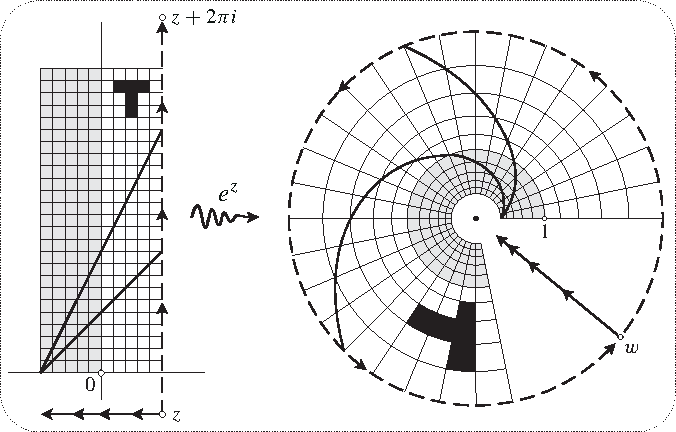
\includegraphics[width=1\textwidth]{needham_figure.pdf}
    \caption[Eksponentne preslikave]{Eksponentna preslikava, po knjigi \cite{Needham_1997}.}
    \label{fig:exponential}
\end{figure}
Dobro vizualizacijo kompleksnega eksponenta nam nudi slika \ref{fig:exponential}, na kateri je \(w = e^z\). Na neformalen način navedemo naslednja opažanja.
\begin{itemize}
    \item Če točka \(z\) potuje navzgor s hitrostjo \(v\), potem se točka \(w\) vrti okrog izhodišča s kotno hitrostjo \(v\). Ko \(z\) prepotuje razdaljo \(2 \pi\), \(w\) enkrat zaokroži okoli izhodišča. Torej je preslikava periodična s periodo \(2 \pi i\).
    \item Če točka \(z\) potuje proti levi s konstantno hitrostjo, točka \(w\) potuje proti izhodišču s pojemajočo hitrostjo. Obratno, če \(z\) potuje proti desni, potem \(w\) potuje stan od izhodišča s pospešeno hitrostjo.
    \item Po prejšnjih dveh alinejah bo celo \(w\)-ravnino brez točke \(w = 0\) pokril vodoraven pas višine \(2 \pi\) v \(z\)-ravnini.
    \item Vodoravne premice se preslikajo v žarke iz izhodišča, v posebnem se realna os preslika v \([0, \infty)\). Navpične črte se preslikajo v krožnice okrog izhodišča, v posebnem se imaginarna os preslika v enotsko krožnico. Splošna premica se preslika v spiralo, ki se navija okrog izhodišča.
    \item Sivo obarvana leva polravnina se preslika v enotski disk, desna polravnina pa v njegov komplement.
    \item Slike majhnih koordinatnih kvadratov ostanejo homeomorfne kvadratom, pri čemer se krožnice s poltraki sekajo pod pravim kotom. To ponazarja, da je preslikava konformna---ohranja kote.
\end{itemize}

\subsection{Hiperbolična geometrija}

Temelj evklidske geometrije nam postavi pet Evklidovih aksiomov.
\begin{enumerate}
    \item Skozi poljubni dve točki poteka natanko ena premica.
    \item Premica je neomejena.
    \item Za vsako daljico obstaja krožnica, ki ima to daljico za polmer in eno od krajišč za središče.
    \item Vsi pravi koti so skladni.
    \item Za poljubno premico \(p\) in točko \(A\), ki ne leži na premici \(p\), obstaja natanko ena premica \(q\), ki vsebuje \(A\) in ne seka premice \(p\).
\end{enumerate}

\noindent Zadnji peti aksiom se imenuje \emph{aksiom o vzporednici}. V hiperbolični geometriji ga nadomestimo z

\begin{enumerate}[resume]
    \item[5'.] Obstajata premica \(p\) in točka \(A\), ki ne leži na premici \(p\), tako da obstajata vsaj dve premici \(q\) in \(r\), ki vsebujeta \(A\) in ne sekata premice \(p\).
\end{enumerate}

\noindent Nov aksiom prinaša veliko posledic, med drugim tudi drugo metriko; \emph{hiperbolično metriko}, katere lastnosti bomo uporabili pri dokazu. Metriko najprej definiramo na enotskem disku \(\DD\) in jo nato razširimo na bolj splošne množice. Poglavje je povzeto po članku \cite[razdelek 3]{Shen_2015}.

Hiperbolično metriko podamo prek \emph{hiperboličnega ločnega elementa} najprej na enotskem disku:
\[\dd \rho_{\DD} (z) = \frac{2 |\dd z|}{1 - |z|^2}.\]
Hiperbolični ločni element nam pove, da se infinitezimalna sprememba v točki \(z\) v hiperbolični metriki izrazi kot infinitezimalna sprememba v evklidski metriki, pomnožena s t.i.~\emph{gostoto} hiperbolične metrike
\[\rho_{\DD} (z) = \frac{2}{1 - |z|^2}.\]
Iz tega izhaja naslednja definicija.

\begin{definicija}
    Naj bo \(\gamma \colon [a, b] \to \DD\) odsekoma \(C^1\) krivulja. Njena \emph{hiperbolična dolžina} je
    \[l_{\DD} (\gamma) \coloneq \int_{\gamma} \rho_{\DD} (z) \, | \dd z | = \int_{a}^{b} \frac{2 | \gamma' (t) | }{1 - | \gamma (t) |^2} \, \dd t.\]
\end{definicija}

\noindent Končno hiperbolično metriko definiramo kot sledi.

\begin{definicija}
    \emph{Hiperbolična metrika} je preslikava \(d_{\DD} \colon \DD \times \DD \to [0, \infty)\), definirana kot
    \[d_{\DD} (z, w) \coloneq \inf_{\gamma} l_{\DD} (\gamma),\]
    kjer \(\gamma\) teče po vseh odsekoma \(C^1\) krivuljah v \(\DD\), ki povezujejo točki \(z\) in \(w\).
\end{definicija}

Definicijo nam iz enotskega diska na enostavno povezana območja prenese naslednji izrek, katerega dokaz najdemo v delu \cite[izrek 6.4]{Beardon_2006}.

\begin{izrek}[Pick] \label{thm:pick}
    Naj bosta \(U, V \subsetneq \CC\) enostavno povezani območji in \(f \colon U \to V\) holomorfna preslikava. Potem na \(U\) obstaja enolično določena gostota hiperbolične metrike \(\rho_U\), da veljajo naslednje izjave.
    \begin{enumerate}
        \item Za vsak \(z \in \DD\) velja \(\rho_{\DD} (z) = \frac{2}{1 - |z|^2}\).
        \item Preslikava \(f\) ne veča \emph{hiperboličnega odvoda}, to pomeni, da velja \[\hder{f (z)}{U}{V} \coloneq |f' (z)| \cdot \frac{\rho_V (f (z))}{\rho_U (z)} \leq 1.\]
        \item Enakost \(\hder{f (z)}{U}{V} = 1\) velja natanko tedaj, ko je \(f\) biholomorfna.
        \item Če je \(U \subsetneq V\), potem za vsak \(z \in U\) velja \(\rho_U (z) > \rho_V (z)\).
    \end{enumerate}
\end{izrek}

\noindent S pomočjo druge in tretje točke lahko izračunamo gostoto hiperbolične metrike eksplicitno. To je prikazano v naslednji trditvi.

\begin{trditev}[Zgledi hiperboličnih metrik] \label{prop:hypexamples} \mbox{}
    \begin{enumerate}
        \item Za desno polravnino \(\HH \coloneq \set{ z \in \CC : \re (z) > 0 }\) je \(\displaystyle \rho_\HH = \frac{1}{\re (z)}\).
        \item Za zgornjo polravnino \(\KK \coloneq \set{z \in \CC : \im (z) > 0}\) je \(\displaystyle \rho_{\KK} (z) = \frac{1}{\im (z)}\)
        \item Za pas \(S \coloneq \set{z \in \CC : |\im (z)| < \pi}\) je \(\displaystyle \rho_{S} = \frac{1}{2 \cos (\im (z) / 2)}\).
        \item Za zarezani ravnini velja
              \[
                  \rho_{\CC \setminus [0, \infty)} (z) = \frac{1}{2 |z| \sin (\arg (z) / 2)},
                  \qquad
                  \rho_{\CC \setminus (-\infty, 0]} (z) = \frac{1}{2 |z| \cos (\Arg (z) / 2)}.
              \]
    \end{enumerate}
\end{trditev}

\begin{dokaz}
    Uporabimo izrek \ref{thm:pick} na štirih biholomorfnih funkcijah. Naj bo \(\varphi_1 \colon \HH \to \DD\); \(z \mapsto (1 - z) / (1 + z)\). Potem je
    \[\rho_{\HH} (z) = \rho_{\DD} (\varphi_1 (z)) \cdot \abs{\varphi_1' (z)} = \frac{2}{1 - |\varphi_1 (z)|^2} \cdot \frac{2}{|z + 1|^2} = \frac{4}{|1 + z|^2 - |1- z|^2}.\]
    Za \(z = x + i y\) razpišemo \(|1 \pm z|^2 = 1 \pm 2x + x^2 + y^2\) in dobimo želen rezultat.

    Naj bo \(\varphi_2 (z) \colon \KK \to \DD\); \(\varphi_2 (z) = (z - i) / (z + i)\). Potem po zgornjem postopku dobimo
    \[\rho_{\KK} (z) = \rho_{\DD} (\varphi_2 (z)) \cdot \abs{\varphi_2' (z)} = \frac{4}{|z + i|^2 - |z - i|^2} = \frac{1}{\im (z)}.\]

    \noindent Naj bo \(\varphi_3 \colon S \to \HH\); \(z \mapsto e^{z / 2}\). Potem je
    \[\rho_S (z) = \rho_{\HH} (\varphi_3 (z)) \cdot |\varphi_3' (z)| = \frac{|\varphi_3 (z)|}{2 \re \varphi_3 (z)} = \frac{1}{2 \cos (\arg (\varphi_3 (z)))} = \frac{1}{2 \cos (\im (z) / 2)}.\]
    Zadnja enakost drži, saj iz \(|\im (z)| < \pi\) sledi \(\arg (\varphi_3 (z)) = \im (z) / 2\).

    Naj bo \(\varphi_4 \colon \CC \setminus (- \infty, 0] \to \HH\); \(z \mapsto \sqrt{z}\) glavna veja korena. Ta funkcija je biholomorfna, če se omejimo na rešitev \(r e^{i \theta} \mapsto \sqrt{r} e^{i \theta / 2}\) za \(\theta \in (- \pi, \pi)\). Potem je
    \[\rho_{\CC \setminus (- \infty, 0]} (z) = \rho_{\HH} (\varphi_4 (z)) \cdot |\varphi_4' (z)| = \frac{1}{\re (\sqrt{z})} \cdot \frac{1}{2 |\sqrt{z}|}.\]
    Dobljeno poenostavimo s polarnim zapisom, da dobimo
    \[\frac{1}{2 r \cos (\theta / 2)} = \frac{1}{2 |z| \cos (\Arg (z) / 2)}.\]
    % \[\rho_{\CC \setminus [0, \infty)} (z) = \rho_{\HH} (\varphi_2 (z)) \cdot |\varphi_2' (z)| = \frac{2 |z|}{\re (- z^2)}.\]
    % Uporabimo polarni zapis \(z = r e^{i \theta}\), da dobimo \(- z^2 = - r^2 e^{2 i \theta}\) in \(\re (- r^2 e^{2 i \theta}) = - r^2 \cos (2 \theta)\). Zato z uporabo formule \(\cos (2 \theta) = \cos^2 \theta - \sin^2 \theta\) dobimo
    % \[\frac{2 |z|}{\re (- z^2)} = \frac{2}{- r \cos (2 \theta)} = \frac{2}{r (\sin^2 \theta - \cos^2 \theta)}\]
\end{dokaz}

\section{Kompleksna dinamika}

\subsection{Kompleksne periodične točke}

\noindent Definicijo privlačne in odbojne točke nam v kompleksni ravnini poenostavi naslednji izrek.

\begin{izrek}
    Naj bo \(f\) cela funkcija in \(z^*\) njena fiksna točka. Potem je \(z^*\) privlačna natanko tedaj, ko je \(|f' (z^*)| < 1\). Dodatno je \(z^*\) odbojna natanko tedaj, ko je \(|f' (z^*)| > 1\).
\end{izrek}

\begin{dokaz}
    Naj bo \(z^*\) privlačna. Ker za vsak \(z \in \Delta (z^*, r)\) zaporedje \(f^n (z)\) enakomerno konvergira proti \(z^*\), obstaja \(n_0 \in \NN\), tako da \(|f^n (z) - z^*| < r\) za vsak \(z \in \Delta (z^*, r)\) in \(n \geq n_0\). Opazujemo funkcijo \(\phi (z) = (z - z^*) / r\), ki za vsak \(n \geq n_0\) konjugira \(f^n\) in \(F_n \coloneq \phi \circ f^n \circ \phi^{-1}\). Ko poenostavimo dobimo
    \[F_n (w) = \frac{f^n (r w + z^*) - z^*}{r},\]
    kjer je vsaka \(F_n\) definirana na \(\DD\), ima vrednosti v \(\overline{\DD}\) in zadošča \(F_n (0) = 0\). Schwarzova lema nam pove, da je \(|F_n' (0)| \leq 1\). Recimo, da velja \(|F_n' (0)| = 1\). Spet po Schwarzovi lemi je \(F_n\) rotacija, torej \(F_n (w) = a_n w\) za \(|a_n| = 1\). Tedaj velja
    \[\abs{F_n (w)} = \abs{w} = \frac{\abs{f^n (r w + z^*) - z^*}}{r}\]
    ali ekvivalentno \(\abs{f^n (z) - z^*} = \abs{z - z^*}\) za vsak \(z \in \Delta (z^*, r)\). Ker to pomeni, da \(f^n (z)\) ne konvergira proti \(z^*\), smo prišli do protislovja.

    Obratno, naj obstaja \(k \in \RR\), da vejla \(|f' (z^*)| < k < 1\). Iz definicije odvoda sledi, da obstaja \(r > 0\), da za vsak \(z \in \Delta (z^*, r)\) z \(z \neq z^*\) velja
    \[\abs{\frac{f (z) - f (z^*)}{z - z^*}} < k.\]
    To je ekvivalentno \(|f (z) - z^*| \leq k |z - z^*|\). Induktivno nato pokažemo, da velja \(|f^n (z) - z^*| \leq k^n |z - z^*|\) za \(z \in \Delta (z^*, r)\) in \(z \neq z^*\). Ker je \(\lim_{n \to \infty} k^n = 0\), je \(z^*\) res privlačna.

    Naj bo sedaj \(z^*\) odbojna. Iz zgornjega dokaza vemo, da velja \(|f' (z^*)| \geq 1\). Ker \(|f' (z^*)| \neq 0\), je \(f\) lokalni biholomorfizem na neki okolici točke \(z^*\). Torej lahko izberemo kompaktno okolico \(V\) točke \(z^*\), na kateri je \(f\) biholomorfna, \(z^*\) pa točke v \(V\) odbije, torej njihove orbite divergirajo iz \(V\). Za vsak \(k \in \NN\) nato definiramo
    \[V_k \coloneq V \cap f^{-1} (V) \cap \cdots \cap f^{- k} (V).\]
    Vsaka \(V_k\) je kompaktna okolica \(z^*\), ki vsebuje vse točke \(z\), za katere \(f^j (z) \in V\) za \(1 \leq j \leq k\). Če označimo \(V_0 = V\), je zaporedje \((V_k)_{k \geq 0}\) padajoče zaporedje kompaktnih množic z \(\bigcap_k V_k = \set{z^*}\). Poleg tega iz definicije \(V_k\) sledi zveza \(f (V_k) = V_{k - 1} \cap f (V)\). Ker obstaja \(k_0 \in \NN\), tako da za vsak \(k \geq k_0\) velja \(V_k \subset f (V)\), velja tudi \(f (V_k) = V_{k - 1}\) za \(k \geq k_0\). Izberemo torej \(r > 0\), da \(\Delta (z^*, r) \subset V_{k_0}\) in tak \(h > k_0\), da je \(V_h \subset \Delta (z^*, r / 2)\). Z \(g\) označimo \((h - k_0)\)-to iteracijo \(f^{-1}\), to je \(g = (f^{-1})^{h - k_0}\). Tedaj vidimo, da velja
    \[g \prt{\Delta (z^*, r)} \subset V_h \subset \Delta (z^*, r).\]
    Ker sta \(\Delta (z^*, r)\) in \(g \prt{\Delta (z^*, r)}\) enostavno povezani območji, lahko uporabimo Schwarzovo lemo, ki nam pove, da je \(|g' (z^*)| < 1\). Ker velja \(g' (z^*) = (1 / f' (z^*))^{h - k_0}\), je res \(|f' (z^*)| > 1\).

    Obratno, naj obstaja \(k > 1\), da velja \(|f' (z^*)| > k\). Podobno kot prej obstaja \(r > 0\), da je \(|f (z) - f (z^*)| \geq k |z - z^*|\) za vsak \(z \in \Delta (z^*, r)\) in \(z \neq z^*\). Recimo, da obstaja \(z_0\), da velja \(f^n (z_0) \in \Delta (z^*, r)\) za vsak \(n \in \NN\). Tedaj lahko induktivno pokažemo, da velja \(|f^n (z_0) - z^*| \geq k^n |z_0 - z^*|\). Ker je \(\lim_{n \to \infty} k^n = \infty\), smo prišli do protislovja. Torej je \(z^*\) res odbojna.
\end{dokaz}

\noindent V luči zgornjega izreka lahko definicijo razširimo.

\begin{definicija}
    Naj bo \(U \subseteq \CC\) odprta in \(f \colon U \to \CC\) holomorfna. Naj bo \(w \in U\) fiksna točka preslikave \(f\). Število \(\lambda \coloneq f' (w)\) imenujemo \emph{multiplikator preslikave \(f\) v točki \(w\)}. Fiksna točka \(w\) je
    \begin{itemize}
        \item \emph{superprivlačna}, če je \(\lambda = 0\);
        \item \emph{privlačna}, če je \(|\lambda| < 1\);
        \item \emph{odbojna}, če je \(|\lambda| > 1\);
        \item \emph{racionalno nevtralna}, če je \(|\lambda| = 1\) in \(\lambda^n = 1\) za kak \(n \in \NN\);
        \item \emph{iracionalno nevtralna}, če je \(|\lambda| = 1\) in \(\lambda^n \neq\) za vsak \(n \in \NN\).
    \end{itemize}
\end{definicija}

\begin{definicija}
    Naj bo \(z^*\) fiksna točka preslikave \(f\). Množico
    \[\Omega (f, z^*) \coloneq \set{z_0 \in \CC : \lim_{n \to \infty} f^n (z_0) = z^*}\]
    imenujemo \emph{območje privlaka \(z^*\)}.
\end{definicija}

Množica \(A\) je za funkcijo \(f\) \emph{naprej invariantna}, če je \(f (A) = A\), in \emph{nazaj invariantna}, če je \(f^{-1} (A) = A\). Če je množica naprej in nazaj invariantna, pravimo, da je \emph{popolnoma invariantna}.

\begin{izrek}
    Naj bo \(f\) cela funkcija in \(z^*\) njena privlačna fiksna točka. Potem je \(\Omega (f, z^*)\) odprta in popolnoma invariantna.
\end{izrek}

\begin{dokaz}
    Naj bo \(a \in \Omega (f, z^*)\) in \(r > 0\), da je \(\overline{\Delta (z^*, 2r)} \subset \Omega (f, z^*)\). Ker \(f^n (a)\) konvergira k \(z^*\), obstaja \(k \in \NN\), da je \(|f^k (a) - z^*| < r\). Ker je \(f\) zvezna, obstaja \(\delta > 0\), da je \(|f^k (a) - f^k (z)| < r\) za vsak \(z \in \Delta (a, \delta)\). Potem je
    \[|f^k (z) - z^*| \leq |f^k (z) - f^k (a)| + |f^k (a) - z^*| \leq 2r\]
    za \(|z - a| < \delta\). Torej je \(f^k (z)\) vsebovana v \(\overline{\Delta (z^*, 2r)}\). Zaradi tega je \(\lim_{n \to \infty} f^{k + n} (z) = z^*\) za vsak \(z \in \Delta (a, \delta)\). Torej je \(\Delta (a, \delta) \subset \Omega (f, z^*)\).

    Naj bo \(z_0 \in \Omega (d, z^*)\). Potem
    \[\lim_{n \to \infty} f^n \prt{f (z_0)} = \lim_{n \to \infty} f^{n + 1} (z_0) = z^*\]
    in \(f (z_0) \in \Omega(f, z^*)\). Enako sklepamo, da \(f (z_0) \in \Omega (f, z^*)\) implicira \(z_0 \in \Omega (f, z^*)\).
\end{dokaz}

\noindent Komponenta za povezanost \(\Omega (f, z^*)\), ki vsebuje \(z^*\), se imenuje \emph{neposredno območje privlaka} \(z^*\). Označimo ga z \(\Omega_0 (f, z^*)\).

\begin{trditev} \label{prop:privlak}
    Naj bo \(f\) cela funkcija in \(\Omega \subsetneq \CC\) enostavno povezano območje, ki je popolnoma invariantno za \(f\). Če je \(z^{*} \in \Omega\) privlačna fiksna točka \(f\), potem je \(\Omega\) vsebovana v neposrednem območju privlaka \(z^*\).
\end{trditev}

Posvetimo se še nefiksnim periodičnim točkam. Če je \(z_0\) \(p\)-periodična, potem so vse točke \(z_0, f (z_0), f^2 (z_0), \dots, f^{p - 1} (z_0)\) fiksne točke preslikave \(f^p\). Pišemo \(z_j = f^j (z_0)\) in uporabimo verižno pravilo:
\[(f^p)' (z_j) = f' \prt{f^{p - 1} (z_j)} f' \prt{f^{p - 2} (z_j)} \dots f' \prt{f (z_j)} f' (z_j) = \prod_{k = 0}^{p - 1} f' (z_k).\]
To pomeni, da imajo vse točke \(z_j\) isti multiplikator \(K\). Če je \(K < 1\), potem rečemo, da je \(p\)-cikel privlačen. Če pa je \(K > 1\), rečemo, da je \(p\)-cikel odbojen.

\subsection{Normalne družine}

Naj bosta \(X\) in \(Y\) topološka prostora. Množico zveznih preslikav \(f \colon X \to Y\) opremimo s kompaktno-odprto topologijo. Tedaj relativno kompaktnim množicam pravimo \emph{normalne družine}. V tem poglavju jih bomo prek topologije enakomerne konvergence po kompaktih definirali za holomorfne funkcije na nekem območju \(D \subseteq \CC\). Vemo namreč, da sta zgornji topologiji na metričnih prostorih enaki.
\begin{definicija}
    Zaporedje holomorfnnih funkcij \((f_n)\) na območju \(D \subseteq \CC\) konvergira k \(f\) \emph{enakomerno po kompaktih}, če za vsako kompaktno podmnožico \(K \subset D\) in vsak \(\varepsilon > 0\) obstaja obstaja \(n_0 \in \NN\), da za \(n \geq n_0\) velja \(|f_n (z) - f(z)| < \varepsilon\) za vse \(z \in K\).
\end{definicija}

\begin{primer} \label{ex:primer}
    Zaporedje \(f_n \colon \DD \to \CC\), \(f_n (z) = z^n\) konvergira k \(f \equiv 0\) enakomerno po kompaktih. Res, naj bo \(K \subset \DD\) kompaktna. Tedaj obstaja \(r < 1\), da za vsak \(z \in K\) velja \(|z| < r\). Zato velja
    \[\abs{f_n (z) - f (z)} = \abs{z^n - 0} < r^n.\]
    Trditev sledi, saj je za vsak \(\varepsilon > 0\) tudi \(r^n < \varepsilon\) za dovolj velik \(n\).
\end{primer}

\noindent Naslednji izrek nam pove, da je konvergenca enakomerno po kompaktih v družini holomorfnih funkcij smiselna, saj ohranja holomorfnost.

\begin{izrek}
    Naj bo \((f_n)\) zaporedje holomorfnih funkcij na območju \(D \subseteq \CC\), ki konvergira k \(f\) enakomerno po kompaktih. Potem je tudi \(f\) holomorfna na \(D\).
\end{izrek}

\begin{dokaz}
    Naj bo \(\overline{\Delta (a, r)} \subseteq D\). Ker je \(\overline{\Delta (a, r)}\) kompaktna, zaporedje \(f_n\) tu enakomerno konvergira proti \(f\). Poleg tega vsaka funkcija \(f_n\) za vsak \(z \in \Delta (a, r)\) zadošča Cauchyjevi integralski formuli
    \[f_n (z) = \frac{1}{2 \pi i} \int_{\partial \Delta (a, r)} \frac{f_n (w)}{w - z} \, \dd w.\]
    Ker je konvergenca enakomerna, lahko zamenjamo limito in integral
    \[f (z) = \lim_{n \to \infty} f_n (z) = \lim_{n \to \infty} \frac{1}{2 \pi i} \int_{\partial \Delta (a, r)} \frac{f_n (w)}{w - z} \, \dd w = \frac{1}{2 \pi i} \int_{\partial \Delta (a, r)} \frac{f (w)}{w - z} \, \dd w.\]
    Funkcijo na desni lahko razvijemo v vrsto okoli \(z = a\) in zato je holomorfna na \(\Delta (a, r)\). Torej je taka tudi \(f\).
\end{dokaz}

\begin{definicija}
    Naj bo \(\FFF\) družina holomorfnih funkcij na območju \(D \subseteq \CC\). Pravimo, da je družina \emph{normalna}, če za vsako zaporedje funkcij \((f_n) \subset \FFF\) obstaja podzaporedje \((f_{n_k})\), ki konvergira enakomerno po kompaktih k neki \(f \in \FFF\) ali pa k \(f \equiv \infty\).
\end{definicija}

\subsection{Fatoujeva in Juliajeva množica}

Pri preučevanju dinamike funkcij, lahko domeno razdelimo na dva množici. Prvi, na kateri je obnašanje funkcije ``predvidljivo'', pravimo Fatoujeva množica, drugi, kjer je obnašanje kaotično, pa pravimo Juliajeva množica. Natančno ju definiramo sledeče.

Za celo funkcijo \(f\) je \emph{Fatoujeva množica} sestavljena iz vseh točk \(z_0\), za katere velja, da je \((f^n)\) normalna na neki okolici točke \(z_0\). Označimo jo z \(F (f)\). Njen komplement \(J (f) \coloneq \CC \setminus F (f)\) je \emph{Juliajeva množica}. Po definiciji vidimo, da je Fatoujeva množica vedno odprta, Juliajeva pa vedno zaprta.

\begin{primer}
    Po primeru \ref{ex:primer} zaporedje iteracij funkcije \(f (z) = z^2\) na \(\DD\) konvergira k \(f \equiv 0\) enakomerno po kompaktih. Podobno premislimo, da na \(\CC \setminus \overline{\DD}\) konvergira k \(f \equiv \infty\) enakomerno po kompaktih. Na \(\partial \DD\) zaporedje divergira. Zato je \(F (f) = \CC \setminus \partial \DD\) in \(J (f) = \partial \DD\).
\end{primer}

\begin{izrek}
    Naj bo \(B (f)\) množica vseh točk \(z \in \CC\) z omejeno orbito. Tedaj velja
    \[\partial (B (f)) \subset J (f).\]
\end{izrek}

\begin{dokaz}
    Naj bo \(z_0 \in \partial (B (f))\). Recimo, da \(z_0 \notin J (f)\). Potem je \((f^n)\) normalna na neki kompaktni okolici \(U\) točke \(z_0\). Ker je točka \(z_0\) robna, obstajata \(z_1, z_2 \in U\), tako da je orbita točke \(z_1\) omejena, orbita točke \(z_2\) pa ne. Torej ima \((f^n (z_n))\) divergentno podzaporedje \((f^{n_k} (z_2))_k\). Ker pa je \((f^n)\) normalna na \(U\), obstaja podzaporedje zaporedja \((f^{n_k} (z_2))_k\), ki enakomerno konvergira na \(U\). Ker je \((f^n (z_1))\) omejena in \((f^{n_k} (z_2))_k\) divergira k \(\infty\), smo prišli do protislovja.
\end{dokaz}

\noindent Če na tem mestu upoštevamo izrek \ref{thm:orbits}, hitro vidimo, da je za kompleksno eksponentno preslikavo \(J (f) = \CC\) in \(F (f) = \emptyset\). To pa ne drži tudi za poljubno celo funkcijo. Če za primer navedemo \(f (z) \coloneq (e^z - 1) / 4\), potem \((f^n)\) na \(\DD\) konvergira proti \(0\) enakomerno po kompaktih. Torej Fatoujeva množica vsebuje cel enotski disk.

Kot zanimivost omenimo, da za polinome velja enakost \(\partial (B (f)) = J (f)\). V tem primeru zato množici \(B (f)\) pravimo \emph{napolnjena Juliajeva množica}. Posledično je zgornji izrek uporaben za vizualizacijo Juliajeve množice. Na njem temelji na primer \emph{algoritem vzvratne iteracije}. Slike, ki nastanejo, pa so pogosto zanimive, kot vidimo na sliki \ref{fig:julia}. Tu je upodobljena Juliajeva množica funkcije \(z^2 + c\) za \(c \approx \complexnum{-0.5125+0.5213i}\). Z modro in zeleno barvo obarvana obnočja so Fatoujeva množica, medtem ko so rumeno obarvana območja Juliajeva množica.
\begin{figure}
    \centering
    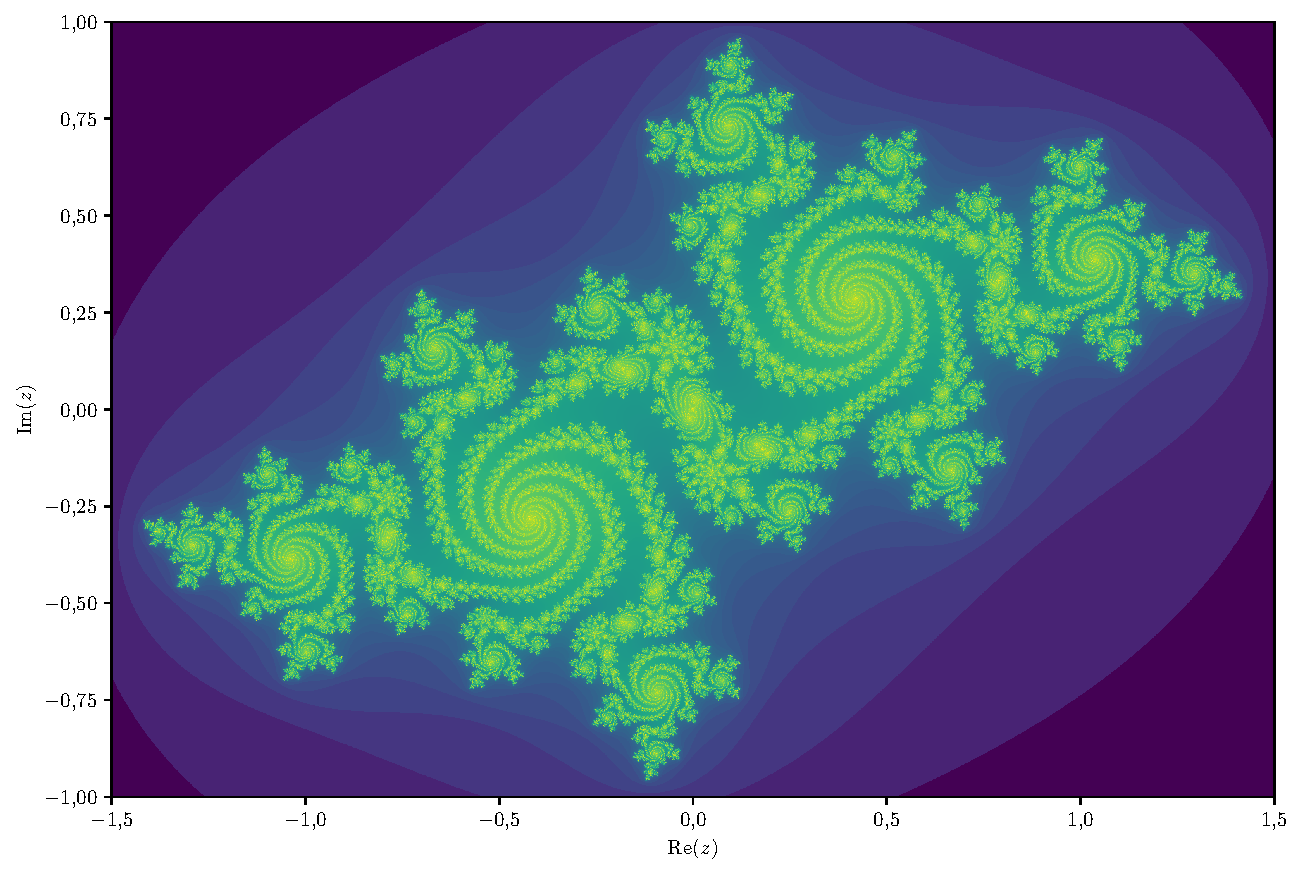
\includegraphics[width=1\textwidth]{julia_set.pdf}
    \caption[Juliajeva množica]{Juliajeva množica funkcije \(z^2 + c\), koda prirejeno po \href{https://commons.wikimedia.org/w/index.php?curid=75993344}{Wikipedia Commons}.}
    \label{fig:julia}
\end{figure}

\input{vsebina/05-gostota_ubeznih.tex}
\input{vsebina/06-tranzitivnost.tex}
\input{vsebina/07-periodicne.tex}
\section{Družina \texorpdfstring{\(\lambda e^z\)}{\lambda exp(z)}}

Dokazali smo, da je \(e^z\) kaotična na celi kompleksni ravnini. Zanimivo pa je, da to ne drži nujno že, če preslikavo pomnožimo s konstanto. V tem poglavju bomo preučili dinamiko \emph{eksponentne družine}
\[E_\lambda (z) \coloneq \lambda e^z.\]
Za \(0 < \lambda < 1/e\) bomo poiskali Juliajevo množico \(J (E_\lambda)\). Poglavje je povzeto po knjigi~\cite[poglavje 9]{Pineiro_2025}.

\subsection{Periodične točke}

Začnemo s preučevanjem realnih fiksnih točk za \(\lambda \in \RR\).

\begin{trditev}
    Naj bo \(\lambda \in \RR\). Potem o realnih fiksnih točkah eksponentne družine lahko povemo naslednje.
    \begin{enumerate}[label=(\arabic*)]
        \item Če je \(\lambda = 1/e\), ima \(E_\lambda\) eno realno fiksno točko \(x^* = 1\).
        \item Če je \(\lambda > 1/e\), potem \(E_\lambda\) nima realnih fiksnih točk.
        \item Če je \(0 < \lambda < 1/e\), potem ima \(E_\lambda\) dve realni fiksni točki: \(x^* \in (0, 1)\) (privlačna) ter \(x^{**} > 1\) (odbojna).
        \item Če je \(\lambda < 0\), potem ima \(E_\lambda\) eno realno fiksno točko \(x^*\):
              \begin{itemize}
                  \item \(x^*\) je privlačna za \(-e < \lambda < 0\);
                  \item \(x^*\) je odbojna za \(\lambda < -e\);
                  \item \(x^*\) je nevtralna za \(\lambda = 1\).
              \end{itemize}
    \end{enumerate}
\end{trditev}

\begin{dokaz}
    (1) Naj bo \(\lambda = 1/e\). Potem je \(E_\lambda (1) = e/e = 1\). Ker je \(E_\lambda' (x^*) = \lambda e^{x^*} = x^* = 1\), je to nevtralna fiksna točka. Ker je premica \(y = ex\) tangenta na \(y = e^x\) v točki \(x = 1\), drugih fiksnih točk ni.

    (2) Naj bo \(\lambda > 1/e\). Pokažemo, da je \(f (x) = \lambda e^x - x > 0\) za vsak \(x \in \RR\), torej da \(\lambda e^z\) nima fiksnih točk. Za \(x < 0\) je očitno \(f (x) > 0\). Za \(x > 0\) preučimo odvod
    \[f' (x) = \lambda \prt{e^x - \frac{1}{\lambda}}.\]
    Tako je \(f' (x) \leq 0\) za \(0 \leq x \leq \ln (1 / \lambda)\) in \(f' (x) > 0\) za \(x > \ln (1 / \lambda)\). Ker je \(f\) zvezna je \(f (\ln(1/\lambda)) = 1 - \ln (1 / \lambda)\) globalni minimum. Torej za vsak \(x \in [0, \infty)\) velja \(f (x) \geq 1 - \ln (1 / \lambda) > 0\).

    (3) Naj bo \(0 < \lambda < 1/e\). Kot pri točki (2) hitro vidimo, da je \(f\) na \((- \infty, 0)\) pozitivna in negativnih fiksnih točk ni. Na \([0, \infty)\) pa ima \(f\) dve ničli, saj je \(f (1) = \lambda e - 1 < 0\). Ker je za \(x \in (0, 1)\) odvod \(E_\lambda' (x) < 1\), je \(x^*\) privlačna in podobno je \(x^{**}\) odbojna.

    (4) Naj bo \(\lambda < 0\). Potem je \(f' (x) = \lambda e^x - 1 < 0\) za vsak \(x \in \RR\), kar pomeni, da je \(f\) strogo padajoča. Ker je
    \[\lim_{x \to - \infty} f (x) = + \infty \qquad \text{in} \qquad \lim_{x \to + \infty} f (x) = - \infty\]
    ima \(f\) natanko eno ničlo, kar pomeni natanko eno fiksno točko \(x^*\) za \(E_\lambda\). Ločimo primere:
    \begin{itemize}
        \item \(-e < \lambda < 0\): v tem primeru \(f (0) = \lambda < 0\) in \(f (-1) = \lambda / e + 1 > 0\) in zato \(x^* \in (-1, 0)\). Ker je \(|E_\lambda' (z^*)| = |E_\lambda (z^*)| < 1\), je privlačna;
        \item \(\lambda < -e\): v tem primeru \(f (-1) = \lambda / e + 1 < 0\) in zato \(z^* \in (- \infty, -1)\). Podobno kot prej je \(|E_\lambda' (z^*)| > 1\) in zato je \(z^*\) odbojna;
        \item \(\lambda = - e\): v tem primeru je \(x^* = -1\) in \(|E_\lambda' (-1)| = 1\).
    \end{itemize}
\end{dokaz}

\noindent Zgornja trditev nam nakaže, da je najbolj zanimiva dinamika v primeru \(0 < \lambda < 1/e\). Temu primeru se bomo v nadaljevanju posvetili. S \(q_\lambda\) označimo privlačno ter s \(p_\lambda\) odbojno točko eksponentne družine.

\begin{lema} \label{lem:enadva}
    Za vsak \(\lambda \in (0, 1/e)\) velja:
    \begin{enumerate}[label=(\arabic*)]
        \item \(q_\lambda < \ln (1 / \lambda) < p_\lambda\);
        \item če je \(l_\lambda \in (\ln (1 / \lambda), p_\lambda)\) realno število, potem je \(E_\lambda (l_\lambda) < l_\lambda\).
    \end{enumerate}
\end{lema}

\begin{dokaz}
    (1) Ker sta \(q_\lambda\) in \(p_\lambda\) fiksni, velja
    \[q_\lambda = E_\lambda (q_\lambda) < 1 = E_\lambda (\ln (1 / \lambda)) < E_\lambda (p_\lambda) = p_\lambda\]
    natanko tedaj, ko
    \[\lambda e^{q_\lambda} < \lambda e^{\ln (1 / \lambda)} < \lambda e^{p_\lambda}\]
    (2) Za \(x \geq 1\) opazujemo funkcijo \(g (x) = e^x / x\). Ker je za \(x > 1\) odvod \(g' (x) > 0\), je \(g\) strogo naraščajoča na \([1, \infty)\). Ker je \(g (1) = e\), \(g (p_\lambda) = 1 / \lambda\) in \(1 < \ln (1 / \lambda) < p_\lambda\), imamo za \(l_\lambda \in (\ln (1 / \lambda), p_\lambda)\) neenakost \(g (l_\lambda) < g (p_\lambda) = 1 / \lambda\).
\end{dokaz}

\begin{trditev} \label{prop:trinajst}
    Naj bo \(\lambda \in (0, 1/e)\) in \(l_\lambda \in (\ln (1 / \lambda), p_\lambda)\).
    \begin{enumerate}[label=(\arabic*)]
        \item Funkcija \(E_\lambda\) preslika polravnino \(\re z < l_\lambda\) samo vase.
        \item Polravnina \(\re z < p_\lambda\) je vsebovana v območju privlaka fiksne točke \(q_\lambda\).
        \item Obstaja \(\mu > 1\), tako da \(|E_\lambda' (z)| \geq \mu\) na celi polravnini \(\re z \geq l_\lambda\).
        \item Na polravnini \(\re z \geq \ln (1 / \lambda)\) je \(|E_\lambda' (z)| > 1\).
        \item Naj bo \(\nu = \ln (1 / \lambda) > 1\) in \(H\) polravnina \(\re z < \nu\). Potem je \(H\) vsebovana v neposrednem območju privlaka točke \(q_\lambda\).
        \item Premica \(\im z = (2n + 1) \pi\) je za vsak \(n \in \ZZ\) vsebovana v
              \[E_\lambda^{-1} \prt{\Omega_0 \prt{E_\lambda, q_\lambda}} \cap \Omega_0 \prt{E_\lambda, q_\lambda}.\]
    \end{enumerate}
\end{trditev}

\begin{dokaz}
    (1) Naj bo \(z\) vsebovan v polravnini \(\re z < l_\lambda\). Po drugi točki leme \ref{lem:enadva} velja
    \[\re \prt{E_\lambda (z)} = \lambda e^{\re z} \cos \prt{\im z} < \lambda e^{l_\lambda} = E_\lambda (l_\lambda) < l_\lambda.\]

    (2) Naj bo \(z\) vsebovan v polravnini \(\re z < p_\lambda\) in \(l_\lambda \in (\ln (1 / \lambda), p_\lambda) \cap (\re z, p_\lambda)\). Po trditvi \ref{prop:privlak}, uporabljeni na polravnini \(\re \zeta < l_\lambda\), vemo, da vsaka z začetno točko v polravnini \(\re \zeta < l_\lambda\) konvergira k \(q_\lambda\).

    (3) Za \(\re z \geq l_\lambda\) velja
    \[|E_\lambda' (z)| = \lambda e^{\re z} \geq \lambda e^{l_\lambda} = \mu > \lambda e^{\ln (1 / \lambda)} = 1.\]

    (4) Slepamo podobno kot v točki (2).

    (5) Opazimo, da \(E_\lambda\) preslika polravnino \(H\) v \(\DD \setminus \{0\}\) in zato \(E_\lambda (H) \subset H\). Po trditvi \ref{prop:privlak} je \(H\) vsebovan v neposrednem območju privlaka točke \(q_\lambda\).

    (6) Če je \(z = x + (2n + 1) \pi i\), potem je \(E_\lambda (z) = - \lambda e^x \in H \subset \Omega_0 (E_\lambda, q_\lambda)\). Po drugi strani je ombočje privlaka popolnoma invariantno in zato \(z \in \Omega (E_\lambda, q_\lambda)\). Ker je množica \(H \cup \set{z : \im z = (2n + 1) \pi}\) povezana, je \(\set{z : \im z = (2n + 1) \pi}\) vsebovana v \(\Omega_0 (E_\lambda, q_\lambda)\).
\end{dokaz}

\begin{posledica} \label{cor:jul-e}
    Za \(\lambda \in (0, 1/e)\), je Juliajeva množica preslikave \(E_\lambda\) vsebovana v polravnini \(\re z \geq p_\lambda\).
\end{posledica}

\begin{posledica}
    Za \(\lambda \in (0, 1/e)\) preslikava \(E_\lambda\) nima nevtralnih fiksnih točk, \(q_\lambda\) pa je edina privlačna fiksna točka.
\end{posledica}

\begin{dokaz}
    Če za \(z_0\) velja \(|(E_\lambda)' (z_0)| \leq 1\), potem je \(\re z_0 \leq \ln (1 / \lambda)\). Torej je \(z_0\) vsebovana v polravnini \(\re z < p_\lambda\). Trditev \ref{prop:trinajst} nam pove, da je vsebovana v območju privlaka točke \(q_\lambda\).
\end{dokaz}

\begin{posledica}
    Za \(\lambda \in (0, 1/e)\) je vsaka periodična točka \(E_\lambda\), ki ni fiksna, odbojna.
\end{posledica}

\begin{dokaz}
    Naj bo \(z_0\) periodična točka \(E_\lambda\) s periodo \(p\) in \(z_0, z_1, \dots, z_{p - 1}\) njena orbita. Vsaka točka \(z_j\) ima periodično orbito, ki zato ni konvergentna. Torej nobena ni vsebovana v polravnini \(\re \zeta < p_\lambda\). Zato \(\re z_j \geq p_\lambda > \ln (1 / \lambda)\). Po tretju točki trditve \ref{prop:trinajst} vemo, da je \(|E_\lambda' (z_j)| > 1\) za \(j = 0, 1, \dots, p - 1\). Po verižnem pravilu izračunamo
    \[\prt{E_\lambda^p}' (z_0) = \prod_{j = 0}^{p - 1} E_\lambda' (z_j),\]
    iz česar vidimo, da velja \(|(E_\lambda^p)' (z_0)| > 1\).
\end{dokaz}

Za konec navedemo dva zanimiva rezultata. Dokaza najdemo v knjigi \cite[trditev 9.1.7, izrek 9.1.8]{Pineiro_2025}.

\begin{trditev}
    Za \(\lambda \in (0, 1/e)\) je območje privlaka točke \(q_\lambda\) gosta podmnožica \(\CC\).
\end{trditev}

\begin{izrek}
    Za \(\lambda \in (0, 1/e)\) je neposredno območje območje privlaka točke \(q_\lambda\) enako Fatoujevi množici \(F (E_\lambda)\), torej \(\Omega_0 (E_\lambda, q_\lambda) = F (E_\lambda)\).
\end{izrek}

\subsection{Juliajeva množica \texorpdfstring{\(E_\lambda\)}{E\_\lambda} za \texorpdfstring{\(0 < \lambda < 1/e\)}{0 < \lambda < 1/e}}

V tem poglavju naj bo vedno \(0 < \lambda < 1/e\). Oznake ostajajo enake kot prej: \(q_\lambda\) in \(p_\lambda\) sta privlačna in odbijajoča točka, za kateri velja \(0 < q_\lambda < 1 < p_\lambda\). Za dan \(\lambda\) in \(l_\lambda \in (\ln (1 / \lambda), p_\lambda)\) bomo v polravnini \(\re z \geq l_\lambda\) konstruirali družino Cantorjevih množic, ki so invariantne za \(E_\lambda\).

Naj bo \(N \in \NN\) označimo
\[B(N) \coloneq \set{x + iy \in \CC : x \in [l_\lambda, r_\lambda], y \in [- (2N + 1) \pi, (2N + 1) \pi]},\]
kjer je \(r_\lambda\) izbran tako, da \(\lambda e^{r_\lambda} > r_\lambda + (2N + 1) \pi\) (glej sliko \ref{fig:konstrukcija}).
\begin{figure}%
    \centering
    \input{tikz/konstrukcija.tex}
    \caption{Ilustracija h konstrukciji.}
    \label{fig:konstrukcija}
\end{figure}
Preslikava \(E_\lambda\) desno stranico pravokotnika \(B (N)\) preslika v krožnico s središčem v izhodišču in polmerom \(\lambda e^{r_\lambda}\), medtem ko se leva stranica preslika v krog s središčem v izhodišču in radijem \(\lambda e^{l_\lambda}\). Oglejmo si kolobar
\[A = \{z : \lambda e^{l_\lambda} \leq |z| \leq \lambda e^{r_\lambda}\}.\]
Dokazali bomo, da ima \(A\) naslednji dve lastnosti.

\vspace{5mm}
\noindent \textbf{Lastnost 1}. Velja \(B (N) \subset \Int (A)\). Res, naj  bo \(z = x + i y \in B (N)\). Po definiciji \(B (N)\) imamo
\[l_\lambda \leq x \leq r_\lambda, \qquad - (2N + 1) \pi \leq y \leq (2N + 1) \pi.\]
Zato
\[|z| \leq |x| + |y| \leq r_\lambda + (2N + 1) \pi < \lambda e^{r_\lambda},\]
kar pomeni, da je \(|z|\) strogo manjše od zunanjega radija \(A\). Po drugi strani pa je
\[|z| \geq l_\lambda > \lambda e^{l_\lambda},\]
torej je \(|z|\) strogo večji od notranjega radija \(A\).

\noindent \textbf{Lastnost 2}. Funkcija \(E_\lambda\) preslika \(B (N)\) v \(A\). Res, naj bo \(z \in B (N)\). Potem \(E_\lambda (z) = \lambda e^x e^{i y}\) in zato
\[|E_\lambda (z)| = \lambda e^x \leq \lambda e^{r_\lambda} \quad \text{in} \quad |E_\lambda (z)| = \lambda e^x \geq \lambda e^{l_\lambda}.\]

Vrnemo se nazaj h konstrukciji. Za vsak \(i = -N, \dots, N\) definiramo `podpravokotnik'
\[R_i \coloneq \set{x + iy \in \CC : x \in [l_\lambda, r_\lambda], y \in [(2i - 1) \pi, (2i + 1) \pi]}.\]
Ker po lastnosti 2 \(E_\lambda\) preslika \(R_i\) v \(A\), ostaja pokazati le, je ta preslikava surjektivna. Naj bo \(w = r \lambda e^{i \theta} \in A\), torej \(r \in (e^{l_\lambda}, e^{r_\lambda})\) in \(\theta \in [(2i - 1) \pi, (2i + 1) \pi]\). Če vzamemo \(x = \ln r\) in postavimo \(z = x + i \theta\), je po definiciji \(z \in R_i\) in
\[E_\lambda (z) = \lambda e^x e^{i \theta} = \lambda r e^{i \theta} = w.\]
Tako je res \(E_\lambda (R_i) = A\). Ker to drži za vsak \(i = -N, \dots, N\), sledi tudi, da je za poljubna \(i, j\): \(R_j \subset E_\lambda (R_i)\).

Po točki (3) trditve \ref{prop:trinajst} obstaja \(\mu > 1\), da velja
\begin{equation} \label{eqn:mu-ocena}
    \bigl| E_\lambda' (z) \bigr| \geq \mu > 1 \quad \text{na polravnini } \re z \geq l_\lambda.
\end{equation}
Zato je ta neenakost izpolnjena tudi na vsakem podpravokotniku \(R_i\). Definiramo
\[\Lambda_N \coloneq \set{z \in B(N) : E_\lambda^j (z) \in B (N) \text{ za vse } j \geq 0},\]
to je množico točk, katerih orbite pod \(E_\lambda\) ostanejo v \(B (N)\). Za vsak \(k = -N, \dots, N\) uvedemo trak
\[S (k) \coloneq \set{x + i y \in \CC : (2k - 1) \pi \leq y \leq (2k + 1) \pi}.\]
Naj bo \(L_k\) veja inverza preslikave \(E_\lambda\), definirana na pozitivno zarezani ravnini \(\CC \setminus [0, \infty)\) tako da
\[L_k (z) = \ln \prt{\frac{|z|}{\lambda}} + i \Arg_k (w),\]
kjer je \(\Arg_k (w) \in [(2k - 1) \pi, (2k + 1) \pi]\). Potem za vsak \(w \in \CC \setminus [0, \infty)\) in \(k = - N, \dots, N\) drži
\begin{equation} \label{eqn:inverz-e}
    E_\lambda \circ L_k (w) = w.
\end{equation}

\begin{trditev} \label{prop:claim}
    Za vsaka \(j, k \in \{-N, \dots, N\}\) velja \(L_k (R_j) \subset \Int (R_k)\).
\end{trditev}

\begin{dokaz}
    Ker je \(R_j \subset A\), lahko vsak \(w \in R_j\) izrazimo kot \(w = r \lambda e^{i \theta}\), kjer je \(r \in (e^{l_\lambda}, e^{r_\lambda})\) in \(\theta \in ((2k - 1) \pi, (2k + 1) \pi)\). Ker je veja inverza \(L_k\) podana z \(L_k (w) = \ln r + i \theta\) dobimo \(L_k (w) \in \Int (R_k)\).
\end{dokaz}

Za nek \(z \in \Lambda_N\) je \(\im (E_\lambda^n (z)) \neq (2j \pm 1) \pi\) za vsak \(n \in \NN\) in vsak \(j = -N, \dots, N\). Res, če je \(E_\lambda^n (z) = x + (2j \pm 1) \pi i\), potem je \(E_\lambda^{n + 1} (z) = - \lambda e^x \notin B (N)\). Zato vsaka točka \(E_\lambda^n (z)\) leži v pravokotniku
\[R_i^* \coloneq \set{x + iy \in \CC : x \in [l_\lambda, r_\lambda], y \in ((2i - 1) \pi, (2i + 1) \pi)},\]
ki ga dobimo, če pravokotniku \(R_i\) odstranimo zgornjo in spodnjo stranico. Tako vsak \(z \in \Lambda_N\) določa svoje natanko določeno zaporedje
\[\overline{s} = (s_0, s_1, s_2, \dots), \qquad s_i \in \{-N, \dots, N\}\]
za katerega velja
\begin{equation} \label{eqn:itinerar}
    E_\lambda^n (z) \in R_{s_n}^* \qquad \text{za vsak } n = 0, 1, \dots
\end{equation}
Zaporedje \(\overline{s}\) imenujemo \emph{itinerar} točke \(z\). Ker je po definiciji veje \(L_{s_n}\) za vsak \(w = E_\lambda^n (z) \in R_{s_n}^*\) prav tako \(L_{s_n} (E_\lambda (w)) = w\) sledi
\begin{equation} \label{eqn:devetpet}
    L_{s_n} \circ E_\lambda \prt{E_\lambda^n (z)} = E_\lambda^n (z).
\end{equation}

V nadaljevanju pokažemo, da za vsak \(\overline{s} \in \Sigma_N\) množica
\[\bigcap_{n \geq 0} L_{s_0} \circ \dots \circ L_{s_{n - 1}} \prt{B (N)} \coloneq \bigcap_{n \geq 1} L_s^{[n]} \prt{B (N)}\]
vsebuje natanko eno točko, ki jo označimo z \(z_{\overline{s}}\). Ker je po trditvi \ref{prop:claim} za vsak \(j, k\)
\[L_k (R_j) \subset \Int (R_k) \implies L_s^{[n + 1]} \prt{B (N)} \subset L_s^{[n]} \prt{B (N)},\]
je zaporedje množic \(\{L_s^{[n]} (B (N))\}_{n = 1}^{\infty}\) padajoče. Da je njihovo presečišče zgolj ena točka, zadostuje, da zaporedje njihovih premerov
\[d_n \coloneq \diam \prt{L_s^{[n]} \prt{B (N)}}\]
konvergira proti \num{0}. Naj bosta \(z_1, z_2 \in B(N)\). Z neenakostjo \(|E_\lambda' (z)| \geq \mu > 1\) (enačba \eqref{eqn:mu-ocena}) in enakostjo \eqref{eqn:devetpet} ter verižnim pravilom dobimo
\[\prt{L_s^{[n]}}' (z) = \prt{E_\lambda^n}' \prt{L_s^{[n]} (z)}^{-1} \implies \abs{\prt{L_s^{[n]}}' (z)} \leq \mu^{- (n + 1)}.\]
Zato velja
\[ \begin{multlined}[12cm]
        \left| L_s^{[n]}(z_2) - L_s^{[n]}(z_1) \right| = \left| \int_{z_1}^{z_2} \prt{L_s^{[n]}}' (z) \, \dd z \right|\\
        \leq |z_2 - z_1| \cdot \sup_{z \in B(N)}\left| \left( L_s^{[n]} \right)'(z) \right| \leq \frac{\diam (B(N))}{\mu^{n+1}}.
    \end{multlined} \]
Ker je \(\mu > 1\), desna stran konvergira proti \num{0} in zato tudi \(d_n\) konvergirajo proti \num{0}.

\begin{izrek}
    Preslikava \(\phi \colon \Sigma_N \to \Lambda_N\); \(\phi (\overline{s}) = z_{\overline{s}}\) je homeomorfizem, ki konjugira skrčitev \(E_\lambda\) na \(\Lambda_N\) ter preslikavo zamika \(\sigma\), torej \(\phi \circ \sigma = E_\lambda \circ \phi\).
\end{izrek}

\begin{dokaz}
    (1) \textbf{Surjektivnost}. Naj bo \(\overline{s} \in \Sigma_N\) itinerar točke \(z \in \Lambda_N\). Z indukcijo pokažemo, da je \(\phi (\overline{s}) = z\). Za \(n = 0\) po definiciji \(z \in B (N)\) velja \(L_{s_0} \circ E_\lambda (z) = z\). Predpostavimo
    \[z = L_{s}^{[n]} \prt{E_{\lambda}^{n + 1} (z)}.\]
    Potem iz enačbe \eqref{eqn:devetpet} in verižnega pravila sledi
    \[L_{s}^{[n + 1]} \prt{E_{\lambda}^{n + 2} (z)} = L_{s}^{[n]} \prt{L_{s_{n + 1}} \circ E_\lambda (E_\lambda^{n + 1} (z))} = L_{s}^{[n]} \prt{E_\lambda^{n + 1} (z)} = z.\]
    S tem smo pokazali, da je \(z \in L_{s_0} \circ L_{s_1} \circ \dots \circ L_{s_n} (B (N))\) za vsak \(n \geq 0\) in zato \(z = \phi (\overline{s})\).

    (2) \textbf{Injektivnost}. Naj bosta \(\overline{s}, \overline{s}^* \in \Sigma_N\), da \(\overline{s} \neq \overline{s}^*\). Naj bo \(j \in \NN\) najmanjši, da je \(s_j \neq s_j^*\). Če bi veljalo \(\phi (\overline{s}) = \phi (\overline{s}^*) = z\), bi po definiciji itinerarja veljalo
    \[E_\lambda^j (z)\in L_{s_j} \prt{B (N)} \cap L_{s_j^*} \prt{B (N)}.\]
    A za \(w \in L_{s_j} \prt{B (N)}\) je imaginarni del \(\im w \in ((2 s_j - 1) \pi, (2 s_j + 1) \pi)\), za \(w^* \in L_{s_j^*} \prt{B (N)}\) pa \(\im w^* \in ((2 s_j^* - 1) \pi, (2 s_j^* + 1) \pi)\). Ker sta ta intervala disjunktna, je to protislovje.

    (3) \textbf{Zveznost}. Naj bo \(\overline{s}^o \in \Sigma_N\) in \(z_0 = \phi (\overline{s}^o)\). Za \(\varepsilon > 0\) izberemo tak \(k\), da
    \[\frac{\diam (B (N))}{\mu^{k + 1}} < \varepsilon,\]
    kjer je \(\mu > 1\) iz ocene \(|E_\lambda'| \geq \mu\) \eqref{eqn:mu-ocena}. Potem ima vsak \(\overline{s}\) iz okolice
    \[U = \set{\overline{s} \in \Sigma_N : s_i = s_i^o \text{ za } 0 \leq i \leq k}\]
    prvih \((k + 1)\) simbolov enakih kot \(\overline{s}^o\). Tako za obe točki \(\phi (\overline{s})\) in \(\phi (\overline{s}^o)\) velja \(\phi (\overline{s}), \phi (\overline{s}^o) \in L_s^{[k + 1]} \prt{B (N)}\). Iz neenakosti v dokazu konvergence premerov \(d_n\) tudi tukaj sledi
    \[\left| \phi (\overline{s}) - \phi (\overline{s}^o) \right| \leq \diam \prt{B (N)} \frac{1}{\mu^{k + 1}} < \varepsilon.\]
    Tako je \(\phi\) zvezna.

    (4) \textbf{Zveznost inverza}. Ker je \(\Sigma_N\) kompakten in \(\phi\) bijektivna, je \(\phi^{-1}\) zvezna.

    (5) \textbf{Konjugacija}. Če je \((s_0, s_1, s_2, \dots) = \phi^{-1} (z)\), potem je \(z \in L_s^{[n]} \prt{B (N)}\) za vsak \(n \in \NN\) in zato \(E_\lambda (z) \in E_\lambda \circ L_s^{[n]} \prt{B (N)}\) za vsak \(n \in \NN\). Uporabimo \eqref{eqn:inverz-e}, da dobimo \(E_\lambda (z) \in L_s^{[n]} \prt{B (N)}\) za vsak \(n \in \NN\). To pomeni \(E_\lambda (z) = \phi (s_1, s_2, \dots) = \phi \circ \sigma (s_0, s_1, s_2, \dots) = \phi \circ \sigma \circ \phi^{-1} (z)\).
\end{dokaz}

\noindent Končno lahko dokažemo enakost
\[\overline{\bigcup_{n \geq 1} \Lambda_N} = J (E_\lambda).\]
Po neenakosti \(|E_\lambda' (z)| \geq \mu > 1\) \eqref{eqn:mu-ocena} za vsak \(z \in \Lambda_N\) in izreku \ref{thm:julm} je \(\Lambda_N \subset J (E_\lambda)\). Ker je \(J (E_\lambda)\) zaprtje množice vseh odbojnih periodičnih točk je dovolj, da dokažemo, da je vaka taka točka v kakšni od množic \(\Lambda_N\). Naj bo \(z_0\) odbojna periodična točka preslikave \(E_\lambda\). S posledico \ref{cor:jul-e} vemo, da \(z \in \{\re z \geq l_\lambda\}\). Periodičen cikel \(\{z_0, E_\lambda (z_0), \dots\}\) je tako omeje na polravnini \(\{\re z \geq l_\lambda\}\), zato je za dovolj velik \(N\) v celoti vsebovan v \(B (N)\). Po definiciji \(\Lambda_N\) so vse točke cikla v \(\Lambda_N\), torej je tudi \(z_0 \in \Lambda_N\).



\end{document}
